\subsection{与主覆叠相伴的覆叠情形}

设 B 为拓扑空间，G 为离散拓扑群，E 为以 G 为群的 B 的主覆叠。记 B-空间 E 的投影为 p。设 b 是 B 的一点，x 是 \(E_{b}\) 的一点。

命题 5. --- 映射 \(h_{(\mathrm{E},x)}\) 从 \(\pi_1(\mathrm{B},b)\) 到 G 出发，将 \(\gamma \in \pi_1(\mathrm{B},b)\) 关联到 G 中的唯一元素 \(g\)，它满足 \(x \cdot g = x \cdot \gamma^{-1}\)，是一个群同态；其核是子群 \(p_*(\pi_1(\mathrm{E},x))\)，它是 \(\pi_1(\mathrm{B},b)\) 的子群。若 E 连通，该同态为满射。

对于每个 \(g \in \mathrm{G}\)，都有 \(h_{(\mathrm{E},x \cdot g)} = \operatorname{Int}(g^{-1}) \circ h_{(\mathrm{E},x)}\)。

设 E 是以 G 为群的 B 的主覆叠，设 x 是 \(E_{b}\) 的一点，并记 E 的投影为 p。对于每个 \(g \in G\)，映射 \(y \mapsto y \cdot g\) 都是 E 的 B-自同构。因此，对于每个 \(g \in G\)、每个 \(y \in E_{b}\) 以及每个 \(\gamma \in \pi_{1}(B, b)\)，都有关系 \((y \cdot g) \cdot \gamma = (y \cdot \gamma) \cdot g\)（参见 III，第 305 页，关系 (4)）。从而，对于 \(\gamma, \delta \in \pi_{1}(B, b)\)，有

\[
\begin{array}{r l} & {x \cdot h _ {(\mathrm{E}, x)} (\gamma \delta) = x \cdot \delta^ {- 1} \gamma^ {- 1}} \\ & {\qquad = (x \cdot h _ {(\mathrm{E}, x)} (\delta)) \cdot \gamma^ {- 1}} \\ & {\qquad = (x \cdot \gamma^ {- 1}) \cdot h _ {(\mathrm{E}, x)} (\delta)} \\ & {\qquad = x \cdot h _ {(\mathrm{E}, x)} (\gamma) h _ {(\mathrm{E}, x)} (\delta),} \end{array}
\]

这证明了 \(h_{(\mathrm{E},x)}\) 是群同态。

其核是 \(x\) 在 \(\pi_1(\mathrm{B}, b)\) 的典范作用下的稳定子，因而根据 III 第 305 页的定理 1 等于 \(p_*(\pi_1(\mathrm{E}, x))\)。映射 \(g \mapsto x \cdot g\) 是从 G 到 \(\mathrm{E}_b\) 的双射。因此，同态 \(h_{(\mathrm{E}, x)}\) 的像是满足下述条件的 \(g \in \mathrm{G}\) 的集合：\(x \cdot g\) 属于 \(x\) 在此作用下的轨道。若 E 连通，则 \(\pi_1(\mathrm{B}, b)\) 在 \(\mathrm{E}_b\) 上传递作用（同上），从而同态 \(h_{(\mathrm{E}, x)}\) 为满射。

令 \(g\in \mathbf{G}\)；对于每个 \(\gamma \in \pi_1(\mathrm{B},b)\)，有

\[
x \cdot g h _ {(\mathrm{E}, x \cdot g)} (\gamma) = (x \cdot g) \cdot \gamma^ {- 1} = (x \cdot \gamma^ {- 1}) \cdot g = x \cdot h _ {(\mathrm{E}, x)} (\gamma) g,
\]

所以 \(h_{(\mathrm{E},x\cdot g)}(\gamma)=g^{-1}h_{(\mathrm{E},x)}(\gamma)g\)。命题得证。

例。--- 1) 设 F 是赋有 G 作用的离散集，令 \(X = E \times^{G} F\) 为与之相伴的 B 的覆叠。记 \(\varphi: E \times F \to X\) 为典范 B-态射。它是覆叠的态射。于是，对于每个 \(\gamma \in \pi_{1}(B, b)\) 和每个 \(f \in F\)，有

\[
\varphi (x, f) \cdot \gamma = \varphi (x \cdot \gamma , f) = \varphi (x \cdot h _ {(\mathrm{E}, x)} (\gamma) ^ {- 1}, f) = \varphi (x, h _ {(\mathrm{E}, x)} (\gamma^ {- 1}) \cdot f).\tag{5}
\]

若将 F 与 \(X_{b}\) 识别，其中所用双射为 \(f \mapsto \varphi(x, f)\)，则右作用 \(\pi_{1}(B, b) \to \operatorname{Aut}(X_{b})^{\circ}\) 是以下三个映射的复合：同态 \(h_{(E,x)}\)、G 到自身的反同态 \(g \mapsto g^{-1}\)，以及由 G 在 F 上的作用诱导的同态 G → Aut(F)。

\begin{enumerate}
\def\labelenumi{\arabic{enumi})}
\setcounter{enumi}{1}
\tightlist
\item
  设 H 是离散拓扑群，设 \(f\colon G\to H\) 是群同态。赋予 H 以 G 的左作用 \(g\cdot h=f(g)h\)，其中 \(g\in G\)、\(h\in H\)。令 \(\mathrm{E}^{\prime}=\mathrm{E}\times^{\mathrm{G}}\mathrm{H}\) 为相伴覆叠；它是以 H 为群的主覆叠（I，第 107 页，例 6）。记 \(q\colon E\times H\to E\times^{G}H\) 为典范映射，并置 \(x^{\prime}=q(x,e)\)。有 \(h_{(E^{\prime},x^{\prime})}=f\circ h_{(E,x)}\)。
\end{enumerate}

事实上，设 \(c\) 是 B 中以 \(b\) 为基点的圈，设 \(\gamma\) 是它在 \(\pi_1(B,b)\) 中的类，并令 \(g = h_{(E,x)}(\gamma)\)；于是有 \(x \cdot \gamma = x \cdot g^{-1}\)。设 \(\widetilde{c}\) 是 E 中起点为 \(x\) 的道路；则 \(t \mapsto q(\widetilde{c}(t), e)\) 是 E' 中起点为 \(x'\) 且提升 B 中道路 \(p \circ \widetilde{c}\) 的道路，所以

\[
x ^ {\prime} \cdot \gamma = q (x \cdot \gamma , e) = q (x \cdot g ^ {- 1}, e) = q (x, f (g) ^ {- 1}) = q (x, e) \cdot f (g) ^ {- 1},
\]

这证明了 \(h_{(\mathrm{E}', x')}(\gamma) = f(g)\)。

\section{同伦与覆叠（局部道路连通空间的情形）}

\subsection{连续映射的同伦提升条件}

命题 1. --- 设 B 是拓扑空间，(E,p) 是 B 的覆叠。设 Y 是拓扑空间，f: Y → B 是连续映射。设 y ∈ Y、x ∈ E、b ∈ B 满足 f(y) = p(x) = b。假设空间 Y 连通且局部道路连通。要存在满足 g(y) = x 的连续提升 g: Y → E，使其提升 f，必要且充分条件是同态 π₁(f,y): π₁(Y,y) → π₁(B,b) 的像包含于同态 π₁(p,x): π₁(E,x) → π₁(B,b) 的像中。

不对空间 Y 作任何假设，该条件仍是必要的。事实上，若这样的提升 g 存在，则有 \(\pi_{1}(f,y)=\pi_{1}(p,x)\circ\pi_{1}(g,y)\)。

证明它是充分的。记 \(s\colon \Lambda_{b}(\mathrm{B})\to \Lambda_{x}(\mathrm{E})\) 为同胚 \(c\mapsto p\circ c\) 的逆同胚（III，第 302 页，命题 3 的推论 2），并令 \(\varphi \colon \Lambda_y(\mathrm{Y})\to \Lambda_x(\mathrm{E})\) 为映射 \(d\mapsto s(f\circ d)\)。映射 \(\varphi\) 连续（I，第 132 页，引理）。

设 \(d\) 和 \(d' \in \Lambda_y(Y)\) 是起点为 \(y\) 且终点相同的道路；证明道路 \(\varphi(d)\) 和 \(\varphi(d')\) 的终点相同。置 \(c = f \circ d\)、\(c' = f \circ d'\)。由于道路 \(d * \overline{d'}\) 是 Y 中以 \(y\) 为基点的圈，道路 \(c * \overline{c'}\) 是 B 中以 \(b\) 为基点的圈，且其类属于同态 \(\pi_1(f, y)\) 的像，因而根据假设属于同态 \(\pi_1(p, x)\) 的像。由命题 4 的推论 2（III，第 303 页），道路 \(s(c * \overline{c'})\) 是 E 中以 \(x\) 为基点的圈。道路 \(s(c' * \overline{c})\) 也如此；由道路提升的唯一性，它等于 \(\overline{s(c * \overline{c'})}\)。因此有 \(s(c' * \overline{c})(\frac{1}{2}) = s(c')(1) = s(c)(1)\)，这正是要证明的。

分别记 \(e_{\mathrm{E}}\colon\Lambda_{x}(\mathrm{E})\to\mathrm{E}\) 和 \(e_{\mathrm{Y}}\colon\Lambda_{y}(\mathrm{Y})\to\mathrm{Y}\) 为终点映射。由于假设空间 Y 连通且局部道路连通，映射 \(e_{Y}\) 是满射且开（III，第 262 页，命题 10）。由上一段，存在唯一的映射 \(g\colon Y\to E\)，使得 \(e_{E}\circ\varphi=g\circ e_{Y}\)。它是连续的，因为映射 \(e_{Y}\) 是严格映射（I，第 18 页，例 2）。

最后，验证映射 g 提升映射 f 且 \(g(y) = x\)。Y 的每一点 z 都是一条起点为 y 的道路 c 的终点。道路 \(\varphi(c)\) 是 \(f \circ c\) 的、起点为 x 且终点为 \(g(z)\) 的提升。因此有 \(p(g(z)) = f(z)\)。当 z = y 且 \(c = e_y\) 时，有 \(\varphi(e_y) = e_x\)，从而 \(g(y) = x\)。

推论 1. --- 设 B 是连通且局部道路连通的拓扑空间，b 是 B 的一点。要使 B 的覆叠 (E, p) 可平凡化，必要且充分条件是：对于纤维 \(E_{b}\) 的每一点 x，同态 \(\pi_{1}(p, x)\) 都是双射。

回顾同态 \(\pi_{1}(p,x)\) 是单射（III，第 303 页，命题 4 的推论 1）。因此，该断言由命题 1 以及 I，第 81 页，命题 6 的推论 4 得出。

注记。--- 设 B 是局部道路连通的拓扑空间，b 是 B 的一点，V 是 b 的开连通邻域，并且从 \(\pi_{1}(V,b)\) 到 \(\pi_{1}(B,b)\) 的同态的像是约化为单位元的子群。由推论 1，B 的每个覆叠在 V 上都可平凡化，因而在 B 的每个包含于 V 的子集上也可平凡化。

推论 2. --- 设 B 是连通且局部道路连通的拓扑空间。若对 B 的某一点 b，群 \(\pi_1(B,b)\) 约化为单位元，则空间 B 单连通。

事实上，由推论 1 立即得到，在这些假设下，B 的每个覆叠都可平凡化。

推论 3. --- 设

\pandocbounded{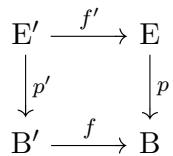
\includegraphics[keepaspectratio]{images/part002_b7191fdb.jpg}}

为笛卡尔方块。假设 E 是 B 的覆叠，且空间 B' 连通并局部道路连通。设 b' 是 B' 的一点，且 \(b = f(b')\)。要使 \((\mathrm{E}', p')\) 成为 B' 的可平凡化覆叠，必要且充分条件是：对于纤维 \(E_b\) 的每一点 x，\(\pi_1(p, x)\) 的像包含 \(\pi_1(f, b)\) 的像。

这由命题 1 以及 I，第 81 页，命题 6 的推论 5 得出。

\subsection{庞加莱群的作用与覆叠的态射}

设 B 是连通且局部道路连通的拓扑空间，b 是 B 的一点。

设 E 是 B 的覆叠。由于假设空间 B 连通，若 E 非空，则纤维 \(E_{b}\) 非空（I，第 74 页，命题 4）。根据 III 第 305 页定理 1 的断言 a)，覆叠 E 连通且非空，当且仅当群 \(\pi_{1}(B,b)\) 在 \(E_{b}\) 上传递作用。

命题 2. --- 设 E 和 E' 是 B 的覆叠。

\begin{enumerate}
\def\labelenumi{\alph{enumi})}
\item
设 \(f\colon\mathrm{E}\to\mathrm{E}^{\prime}\) 是 B-态射。映射 \(f_{b}\colon\mathrm{E}_{b}\to\mathrm{E}_{b}^{\prime}\) 由 \(f\) 导出，分别与 \(\pi_{1}(\mathrm{B},b)\) 在 \(\mathrm{E}_{b}\) 和 \(\mathrm{E}_{b}^{\prime}\) 上的作用相容。当且仅当 \(f\) 是同构时，它是双射。
\item
映射 \(f\mapsto f_{b}\) 是从 B-态射集合 \(\mathcal{C}_{\mathrm{B}}(\mathrm{E};\mathrm{E}^{\prime})\)（其元素是从 E 到 \(\mathrm{E}^{\prime}\) 的 B-态射）到 \(\mathcal{F}_{\pi_1(\mathrm{B},b)}(\mathrm{E}_b;\mathrm{E}_b^{\prime})\)（即 \(\pi_1(\mathrm{B},b)\)-态射集合，其元素是从 \(\mathrm{E}_b\) 到 \(\mathrm{E}_b^{\prime}\) 的态射）的双射。
\end{enumerate}

若 \(f\) 是从 E 到 \(\mathrm{E}'\) 的 B-态射，则映射 \(f_b\colon \mathrm{E}_b\to \mathrm{E}_b'\) 是 \(\pi_1(\mathrm{B},b)\)-态射（参见 III，第 305 页）。此外，两个从 E 到 \(\mathrm{E}'\) 的 B-态射在纤维 \(\mathrm{E}_b\) 上相同，则彼此相等（I，第 80 页，命题 6 的推论 3）。

设 \(\varphi\colon\mathrm{E}_{b}\to\mathrm{E}_{b}^{\prime}\) 是 \(\pi_{1}(\mathrm{B},b)\)-集的态射；证明存在一个 B-态射 \(f\)，它从 E 到 \(\mathrm{E}^{\prime}\) 且满足 \(f_{b}=\varphi\)。不妨设空间 E 和 \(\mathrm{E}^{\prime}\) 连通且非空，于是 \(\mathrm{E}_{b}\) 和 \(\mathrm{E}_{b}^{\prime}\) 是齐性 \(\pi_{1}(\mathrm{B},b)\)-集。设 \(x\) 是 \(\mathrm{E}_{b}\) 的一点；它的稳定子 G 是映射 \(\pi_{1}(p,x)\) 的像（III，第 305 页，定理 1）。由于 \(\varphi\) 是 \(\pi_{1}(\mathrm{B},b)\)-态射，群 G 固定点 \(x^{\prime}=\varphi(x)\)，它属于 \(\mathrm{E}_{b}^{\prime}\)，故 G 包含于映射 \(\pi_{1}(p^{\prime},x^{\prime})\) 的像中。由 III，第 308 页的命题 1，存在一个 B-态射 \(f\)，它从 E 到 \(\mathrm{E}^{\prime}\) 且满足 \(f(x)=x^{\prime}\)。映射 \(f_{b}\) 和 \(\varphi\) 是 \(\pi_{1}(\mathrm{B},b)\)-态射，定义在齐性 \(\pi_{1}(\mathrm{B},b)\)-集 \(\mathrm{E}_{b}\) 到 \(\mathrm{E}_{b}^{\prime}\) 之间，且在点 \(x\) 处相同；所以它们相等。

若 \(f\colon \mathrm{E}\to \mathrm{E}'\) 是 B-同构，则映射 \(f_{b}\colon \mathrm{E}_{b}\to \mathrm{E}_{b}^{\prime}\) 是双射。反之，设映射 \(f_{b}\) 是双射，并令 \(g\colon \mathrm{E}^{\prime}\to \mathrm{E}\) 为满足 \(g_{b} = (f_{b})^{-1}\) 的 B-态射。B-态射 \(g\circ f\colon \mathrm{E}\to \mathrm{E}\) 在 \(\mathrm{E}_b\) 上诱导恒等映射；因此由本命题可知 \(g \circ f = Id_{E}\)。同理，\(f \circ g = Id_{E'}\)，这证明 f 是 B-同构。

推论 1. --- 覆叠 E 和 E' 同构，当且仅当 \(\pi_1(\mathrm{B},b)\)-集 \(\mathrm{E}_b\) 和 \(\mathrm{E}_b'\) 同构。

推论 2. --- 设 (E,p) 和 (E',p') 是 B 的连通覆叠。设 \(x\) 是 \(E_{b}\) 的一点，\(x'\) 是 \(E'_{b}\) 的一点。要存在 B-态射 \(g\colon E\to E'\) 使 \(g(x)=x'\)，必要且充分条件是 \(p_{*}(\pi_{1}(E,x))\subset p'_{*}(\pi_{1}(E',x'))\)。这样的态射唯一；并且当且仅当 \(p_{*}(\pi_{1}(E,x))\) 和 \(p'_{*}(\pi_{1}(E',x'))\) 是 \(\pi_{1}(B,b)\) 的相等子群时，它是同构。

由 III，第 305 页定理 1，从 \(\pi_1(B,b)\) 到 \(E_b\) 的映射由 \(\gamma \mapsto x \cdot \gamma\) 定义，经取商诱导出 \(\pi_1(B,b)\)-集 \(p_*(\pi_1(E,x)) \backslash \pi_1(B,b)\) 到 \(E_b\) 的同构。同样，存在唯一的从 \(\pi_1(B,b)\)-集 \(p'_{*}(\pi_1(E',x')) \backslash \pi_1(B,b)\) 到 \(E_b'\) 的同构。由命题 2，存在一个 B-态射 \(g\colon E\to E'\)，使 \(g(x)=x'\)，当且仅当存在一个 \(\pi_1(B,b)\)-集态射，从 \(p_*(\pi_1(E,x)) \backslash \pi_1(B,b)\) 到 \(p'_{*}(\pi_1(E',x')) \backslash \pi_1(B,b)\)，将类 \(p_*(\pi_1(E,x))\) 送到类 \(p'_{*}(\pi_1(E',x'))\)。这样的态射存在，当且仅当 \(p_*(\pi_1(E,x)) \subset p'_{*}(\pi_1(E',x'))\)。由于假设空间 E 连通，它因而是唯一的（I，第 34 页，命题 11 的推论 2）。当且仅当子群 \(p_*(\pi_1(E,x))\) 和 \(p'_{*}(\pi_1(E',x'))\) 是 \(\pi_1(B,b)\) 的相等子群时，它是同构。

推论 3. --- 设 (E,p) 是 B 的连通覆叠，x 是纤维 \(E_{b}\) 的一点。令 N 表示 \(p_{*}(\pi_{1}(E,x))\) 在 \(\pi_{1}(B,b)\) 中的正规化子。对于 N 的每个元素 \(\gamma\)，存在唯一的 B-自同构 g，使得 \(g(x) = x \cdot \gamma\)；并且映射 \(\gamma \mapsto g\) 经取商定义了从 \(\mathrm{N}/p_{*}(\pi_{1}(\mathrm{E},x))\) 到 \(\mathrm{Aut}_{\mathrm{B}}(\mathrm{E})\) 的群同构。

设 \(\gamma \in \pi_1(\mathrm{B}, b)\)；有 \(p_*(\pi_1(\mathrm{E}, x)) = \operatorname{Int}(\gamma)(p_*(\pi_1(\mathrm{E}, x \cdot \gamma)))\)（III，第 305 页，定理 1，c)）。由推论 2，要存在 B-自同构 \(g\) 使 \(g(x) = x \cdot \gamma\)，必要且充分条件是 \(\gamma\) 属于 N。这样的同构因而唯一。记 \(\alpha: \mathrm{N} \to \mathrm{Aut}_{\mathrm{B}}(\mathrm{E})\) 为由此定义的映射 \(\gamma \mapsto g\)。

设 \(\gamma\) 和 \(\gamma'\) 是 N 的两个元素。置 \(g = \alpha(\gamma)\)、\(g' = \alpha(\gamma')\)；根据关系式 (4)（III，第 305 页）和 (1)（第 304 页），有 \(g(g'(x)) = g(x \cdot \gamma') = g(x) \cdot \gamma' = (x \cdot \gamma) \cdot \gamma' = x \cdot (\gamma\gamma')\)。因此，\(\alpha\) 是群同态。要有 \(\alpha(\gamma) = \mathrm{Id}_{\mathrm{E}}\)，必要且充分条件是 \(x \cdot \gamma = x\)，因为 \(\alpha(\gamma)\) 唯一；也就是说，\(\gamma \in p_*(\pi_1(E, x))\)（III，第 305 页，定理 1，b)）。最后，若 \(g\) 是 E 的 B-自同构，则存在一条道路 \(c\)，它在 E 中连接 \(x\) 与 \(g(x)\)（E 是道路连通的），于是 \(g(x) = x \cdot \gamma\)，其中 \(\gamma\) 是道路 \(p \circ c\) 的类。这证明同态 \(\alpha\) 是满射。

群 \(\mathrm{Aut}_{\mathrm{B}}(\mathrm{E})\) 在纤维 \(\mathrm{E}_b\) 上作用，并被识别为齐性 \(\pi_1(\mathrm{B},b)\)-集 \(\mathrm{E}_b\)（右作用）的自同构群（参见 A，I，第 56 页，命题 5 和 6）。

推论 4. --- 设 (E, p) 是 B 的连通覆叠，x 是纤维 \(E_{b}\) 的一点。要使 E 成为 B 的伽罗瓦覆叠，必要且充分条件是 \(p_{*}(\pi_{1}(E, x))\) 是 \(\pi_{1}(B, b)\) 的正规子群。此时群 \(\mathrm{Aut}_{\mathrm{B}}(\mathrm{E})\) 同构于商群 \(\pi_{1}(\mathrm{B}, b)/p_{*}(\pi_{1}(\mathrm{E}, x))\)。

若 \(p_{*}(\pi_{1}(\mathrm{E},x))\) 是 \(\pi_1(\mathrm{B},b)\) 的正规子群，则根据推论 3，群 \(\mathrm{Aut}_{\mathrm{B}}(\mathrm{E})\) 在纤维 \(\mathrm{E}_b\) 上传递作用，所以 E 是 B 的伽罗瓦覆叠（I，第 102 页，定理 2）。逆命题是 III，第 305 页定理 1 的断言 d)。最后一个断言由推论 3 得出。

\subsection{庞加莱群胚的无局部单值作用}

引理 1. --- 设 B 是局部道路连通的拓扑空间，\(p \colon E \to B\) 和 \(p' \colon E' \to B\) 是满足道路提升性质的平展分离映射（III，第 302 页）。设 \(g \colon E \to E'\) 是满足 \(p' \circ g = p\) 的映射。假设 \(g\) 与群胚 \(\varpi(B)\) 在 \(E\) 和 \(E'\) 上的典范作用相容。则 \(g\) 连续。

设 c 是 E 中的一条道路；置 \(c' = g \circ c\)，并证明映射 \(c'\) 连续。记 B 中的道路 \(p \circ c\) 为 d，并对每个 \(t \in I\)，记 \(d_t\) 为道路 \(s \mapsto d(st)\)。对于所有 \(t \in I\)，有 \(c(t) = c(0) \cdot d_t\)（III，第 304 页，注记 3），由关于 g 的假设，从而有 \(c'(t) = c'(0) \cdot d_t\)，这根据同一注记说明 \(c'\) 是道路 d 的提升。这说明映射 g 按道路连续。由于空间 E 局部道路连通（III，第 261 页，命题 2 的推论 2），映射 g 连续（III，第 269 页，命题 13 的推论）。

设 B 是拓扑空间。考虑一种作用 \(\varphi = (\varphi_{a,b})_{(a,b)\in \mathrm{B}\times \mathrm{B}}\)，它是群胚 \(\varpi (\mathrm{B})\) 关于映射 \(p\colon \mathrm{E}\to \mathrm{B}\) 在集合 E 上的作用。称 \(\varpi (\mathrm{B})\) 在 E 上无单值性地作用，若对每个 \(b\in \mathrm{B}\) 和每个圈类 \(\gamma \in \pi_1(\mathrm{B},b)\)，\(\gamma\) 在纤维 \(\mathrm{E}_b\) 上的作用是平凡的，则称作用 \(\varphi\)（即群胚 \(\varpi (\mathrm{B})\) 的作用）无单值性地作用在 E 上（参见 II，第 168 页）。若 B 道路连通，只需对 B 的一个点验证这一点即可（同上）。如果 B 的每一点都有邻域 V，使得 \(\varpi (\mathrm{V})\) 在集合 \(\mathrm{E_V} = p^{-1}(\mathrm{V})\) 上关于映射 \(p_{\mathrm{V}} = p\mid p^{-1}(\mathrm{V})\) 无单值性地作用，则称群胚的作用无局部单值性。

注记。--- 设 B 是局部道路连通的拓扑空间，并假设 B 的每一点 b 都有邻域 V，使得 \(\pi_{1}(V,b)\) 在 \(\pi_{1}(B,b)\) 中的像约化为单位元（参见 IV，第 340 页，定义 2）。那么，群胚 \(\varpi(B)\) 的每个作用都无局部单值性。

事实上，考虑集合 E、映射 \(p \colon \mathrm{E} \to \mathrm{B}\) 以及作用 \(\varphi\)；它是群胚 \(\varpi(\mathrm{B})\) 关于 \(p\) 在 E 上的作用。设 \(a\) 是 B 的一点，V 是 \(a\) 的邻域，并且 \(\pi_1(\mathrm{V}, a)\) 在 \(\pi_1(\mathrm{B}, a)\) 中的像约化为单位元。设 U 是包含于 V 的 \(a\) 的道路连通邻域。设 \(b\) 是 U 的一点，\(\gamma \in \pi_1(\mathrm{U}, b)\)。设 \(\delta\) 是 U 中连接 \(a\) 与 \(b\) 的道路的类。于是，\(\delta\gamma\delta^{-1}\) 是 U 中以 \(a\) 为基点的圈的类；因此，它在 \(\pi_1(\mathrm{B}, a)\) 中的像是平凡的。从而有 \(\varphi_{a,a}(\delta\gamma\delta^{-1}) = \mathrm{Id}_{\mathrm{E}_a}\)，所以 \(\varphi_{b,b}(\gamma) = \mathrm{Id}_{\mathrm{E}_b}\)。这说明 \(\varpi(\mathrm{U})\) 关于 U-空间 \(\mathrm{E_U}\) 的作用无单值性。因此，作用 \(\varphi\) 无局部单值性。

命题 3. --- 设 B 是局部道路连通的拓扑空间，E 是赋有作用 \(\varphi\)（群胚 \(\varpi(B)\) 的作用）的集合，该作用关于映射 \(p: E \to B\) 无局部单值性。于是 E 上存在唯一的拓扑，使得下列条件成立：

\begin{enumerate}
\def\labelenumi{(\roman{enumi})}
\item
  赋予此拓扑的集合 E 连同映射 p 是 B 的覆叠；
\item
  \(\varpi(\mathrm{B})\) 在此覆叠上的典范作用与作用 \(\varphi\) 相同。
\end{enumerate}

这种拓扑的唯一性由 III，第 312 页的引理 1 得出，其中取 E 的恒等映射作为 g。为证明其存在性，还可假设 B 连通且非空。

首先假设作用 \(\varphi = (\varphi_{a,b})_{(a,b)\in \mathrm{B}\times \mathrm{B}}\) 是群胚 \(\varpi (\mathrm{B})\) 关于 \(p\) 在集合 E 上的无单值作用。

设 \(a\) 是 B 的一点。对于每个 \(b \in \mathrm{B}\)，存在一条道路 \(c\) 在 B 中连接点 \(a\) 与点 \(b\)。若 \(\gamma \in \varpi_{a,b}(\mathrm{B})\) 表示道路 \(c\) 的类，则双射 \(\varphi_{a,b}(\gamma) \colon \mathrm{E}_a \to \mathrm{E}_b\) 与道路 \(c\) 无关，因为该作用无单值性；将此双射记为 \(f_{a,b}\)。映射 \(\Phi_a \colon \mathrm{B} \times \mathrm{E}_a \to \mathrm{E}\)（由 \((b,x) \mapsto f_{a,b}(x)\) 定义）是双射；其逆双射将 \(x \in \mathrm{E}\) 映到二元组 \((p(x), f_{p(x),a}(x))\)。赋予集合 \(\mathrm{E}_a\) 离散拓扑，于是 B-空间 \(\mathrm{B} \times \mathrm{E}_a\) 是 B 的平凡覆叠。通过结构转移，双射 \(\Phi_a\) 在 E 上赋予一个拓扑，使其成为 B 的覆叠。

证明 \(\varpi(\mathrm{B})\) 在 E 上的典范作用与作用 \(\varphi\) 相同。设 \(x\) 是 \(\mathrm{E}_a\) 的一点，设 \(b\) 是 B 的一点。设 \(c\) 是 B 中连接点 \(a\) 与点 \(b\) 的道路；映射 \(t \mapsto \Phi_a(c(t), x)\) 是 E 中连接点 \(x\) 与点 \(\Phi_a(b, x) = f_{a,b}(x)\) 的道路。若 \(\gamma \in \varpi_{a,b}(\mathrm{B})\) 表示道路 \(c\) 的类，则有 \(x \cdot \gamma = f_{a,b}(x)\)。这说明 \(\varpi(\mathrm{B})\) 在覆叠 E 上的典范作用与作用 \(\varphi\) 在起点为 \(a\) 的道路类上相同。由于这些类生成群胚 \(\varpi(\mathrm{B})\)，两个作用相同。

现在处理一般情形。令 \(\mathcal{B}\) 为 E 的开子集 V 的集合，其中 \(\varpi(\mathrm{V})\) 在 \(p^{-1}(\mathrm{V})\) 上无单值性地作用。根据假设，\(\mathcal{B}\) 中的元素覆盖 B。由上文，对于每个 \(\mathrm{V} \in \mathcal{B}\)，在集合 \(p^{-1}(\mathrm{V})\) 上存在唯一拓扑，使得 \((p^{-1}(\mathrm{V}), p_{\mathrm{V}})\) 成为 V 的覆叠，并且 \(\varpi(\mathrm{V})\) 在此覆叠上的典范作用与 \(\varphi\) 诱导的作用相同。

设 \(V' \in \mathcal{B}\)。上面定义的在 \(p^{-1}(V \cap V')\) 上由 \(p^{-1}(V)\) 的拓扑（分别由 \(p^{-1}(V')\) 的拓扑）诱导的拓扑，确实使其成为 \(V \cap V'\) 的覆叠，并且 \(\varpi(V \cap V')\) 在其上的典范作用由作用 \(\varphi\) 诱导。因此这些拓扑都与 \(p^{-1}(V \cap V')\) 的拓扑相同。于是存在 E 上唯一的拓扑，在每个 \(p^{-1}(V)\) 上诱导出先前定义的拓扑（参见 I，§2，第 16 页）。

赋予 E 此拓扑后，映射 p 连续，且 B-空间 E 是覆叠。\(\varpi(\mathrm{B})\) 的典范作用与作用 \(\varphi\) 在像包含于 \(\mathcal{B}\) 中某个开集内的道路类上相同。由引理 4 的

III，第 272 页，这些类生成群胚 \(\varpi(B)\)。因此这两个作用相同（II，第 167 页）。

推论。--- 设 B 是连通且局部道路连通的拓扑空间，(E,p) 是 B-空间，其投影 p 是平展、分离且具有道路提升性质的映射。若 \(\varpi(\mathrm{B})\) 关于 p 在集合 E 上的典范作用无局部单值性，则 E 是 B 的覆叠。

给 E 赋予由道路提升定义的 \(\varpi(B)\) 的典范作用（III，第 303 页，编号 3）。E 上存在一个拓扑，使条件 (i) 和 (ii) 的命题 3 得以满足。根据 III，第 312 页的引理 1，此拓扑与 E 上给定的拓扑相同。

\subsection{庞加莱群的容许拓扑}

设 B 是拓扑空间，\(a\) 是 B 的一点。称 \(\pi_1(B, a)\) 的子群 H 为容许的，如果 B 的每一点 \(b\) 都有邻域 V，使得 \(\gamma i_*(\delta)\gamma^{-1} \in \mathrm{H}\) 对每个 \(\gamma \in \varpi_{a,b}(\mathrm{B})\) 和每个 \(\delta \in \pi_1(V, b)\) 都成立，其中 \(i: V \to B\) 是典范嵌入。如果 H 是 \(\pi_1(B, a)\) 的正规子群，则要使 H 容许，只需对一个道路类 \(\gamma \in \varpi_{a,b}(\mathrm{B})\) 验证此条件即可。

命题 4. — \(\pi_1(B, a)\) 上存在唯一一个与其群结构相容的拓扑，使 \(\pi_1(B, a)\) 的容许正规子群构成单位元的邻域基。在此拓扑下，开子群恰好是容许子群。

由容许子群的定义得到以下事实：

\begin{enumerate}
\def\labelenumi{\alph{enumi})}
\item
  群 \(\pi_1(B, a)\) 是容许的；
\item
  包含某个容许子群的子群是容许的；
\item
  有限个容许子群的交是容许的。
\item
对于 \(\pi_{1}(B,a)\) 的每个容许子群 H，各子群 \(\gamma H\gamma^{-1}\) 的交（其中 \(\gamma\) 遍历 \(\pi_{1}(B,a)\)）是容许的。
\end{enumerate}

特别地，容许正规子群的集合是一个滤基，由 \(\pi_1(B,a)\) 中满足公理 (GV \(_{\text{III}}'\) ) 的子群组成；根据 TG，III，第 5 页，例，这就得到命题的第一部分。第二部分随即显然（参见 TG，III，第 7 页，命题 4 的推论）。

命题 4 所刻画的群 \(\pi_{1}(B,a)\) 上的拓扑称为容许拓扑。

注记。--- 1) 若 B \(_{0}\) 表示 B 中 \(a\) 的道路连通分支，则在这些群赋予容许拓扑时，典范同构 \(\pi_{1}(B_{0}, a) \to \pi_{1}(B, a)\) 是拓扑群同构。

\begin{enumerate}
\def\labelenumi{\arabic{enumi})}
\setcounter{enumi}{1}
\item
设 B 是拓扑空间。设 \(b\) 和 \(b'\) 是属于同一道路连通分支的 B 的点，并设 \(\gamma\) 是 \(\varpi_{b,b'}(B)\) 的元素。由容许子群的定义，对于 \(\pi_1(B,b')\) 的每个容许子群 H，子群 \(\gamma H\gamma^{-1}\) 是 \(\pi_1(B,b)\) 的容许子群。因此，同构 \(u_\gamma \colon \delta \mapsto \gamma \delta \gamma^{-1}\) 从 \(\pi_1(B,b')\) 到 \(\pi_1(B,b)\)（参见 III，第 292 页）在这些群赋予容许拓扑时是同胚。
\item
  设 A 和 B 是拓扑空间，\(a\) 是 A 的一点，\(f\colon\mathrm{A}\to\mathrm{B}\) 是连续映射。置 \(b=f(a)\)。若 H 是 \(\pi_{1}(\mathrm{B},b)\) 的容许子群，则它在同态 \(\pi_{1}(f,a)\) 下的逆像是 \(\pi_{1}(\mathrm{A},a)\) 的容许子群。因此，当这些群赋予容许拓扑时，群同态 \(\pi_{1}(f,a)\colon\pi_{1}(\mathrm{A},a)\to\pi_{1}(\mathrm{B},b)\) 连续。
\end{enumerate}

命题 5. --- 设 B 是局部道路连通的拓扑空间，a 是 B 的一点。要使 \(\pi_1(\mathrm{B},a)\) 的子群 H 容许，必要且充分条件是存在 B 的覆叠 (E,p) 以及一点 \(x\in \mathrm{E}_a\)，使得 \(\mathrm{H} = p_{*}(\pi_{1}(\mathrm{E},x))\)。

设 \((\mathrm{E},p)\) 是 B 的覆叠，设 x 是 \(E_{a}\) 的一点；置 \(\mathrm{H}=p_{*}(\pi_{1}(\mathrm{E},x))\)，并证明它是 \(\pi_{1}(\mathrm{B},a)\) 的容许子群。设 b 是 B 的一点，V 是 b 的邻域，并且 \(\mathrm{E}_{\mathrm{V}}=(p^{-1}(\mathrm{V}),p_{\mathrm{V}})\) 是 V 的可平凡化覆叠。设 \(\gamma\in\varpi_{a,b}(\mathrm{B})\)；证明对于每个 \(\delta\in\pi_{1}(\mathrm{V},b)\)，道路类 \(\gamma\delta\gamma^{-1}\) 属于 H。

由 III，第 301 页命题 3，存在唯一的道路严格同伦类 \(\gamma'\)，其起点为 E 中的 \(x\)，且 \(p_*(\gamma') = \gamma\)。设 \(y\) 是 \(\gamma'\) 的终点；有 \(p(y) = b\)（III，第 302 页，命题 4）。再令 \(\delta'\) 为 E 中起点为 \(y\) 且满足 \(p_*(\delta') = \delta\) 的唯一道路类。由于 \(\mathrm{E_V}\) 可平凡化，\(\delta'\) 是以 \(y\) 为基点的圈的类。于是，\(\gamma'\delta'(\gamma')^{-1}\) 是 E 中以 \(a\) 为基点的圈的类，其在 \(p_*\) 下的像是类 \(\gamma\delta\gamma^{-1}\)，这正是要证明的。

反之，设 H 是 \(\pi_1(B, a)\) 的容许子群。令 \(\lambda_a(B)\) 为对道路严格同伦关系取商所得的空间 \(\Lambda_a(B)\) 的商集，其中道路的起点为 \(a\)；由于严格同伦的道路具有相同的终点，终点映射 \(e: \Lambda_a(B) \to B\) 经取商定义了映射 \(\varepsilon: \lambda_a(B) \to B\)。道路类的复合赋予集合 \(\lambda_a(B)\) 以群 \(\pi_1(B, a)\) 的左作用。将此作用限制为群 H 的作用，并将其轨道集合记为 \(H\backslash\lambda_a(B)\)。

映射 \(\varepsilon\colon\lambda_{a}(B)\to B\) 经取商诱导出映射 \(q\colon H\backslash\lambda_{a}(B)\to B\)。道路类的复合赋予集合 \(H\backslash\lambda_a(B)\) 以群胚 \(\varpi(B)\) 关于映射 \(q\) 的右作用。

此作用无局部单值性。事实上，设 \(b\) 是 B 的一点，V 是 \(b\) 的一个邻域，使得 \(\gamma i_{*}(\pi_{1}(V,b))\gamma^{-1}\subset H\) 对每个道路类 \(\gamma\) 都成立，其中这些道路连接 B 中的 \(a\) 与 \(b\)，而 \(i\) 表示 V 到 B 的嵌入。由于 B 局部道路连通，还可进一步假设 V 道路连通。设 \(c\in V\)，令 \(\delta\) 为 \(\pi_1(B,c)\) 中的、以 \(c\) 为基点且像包含于 V 的圈的类，并令 \(\delta'\) 为 \(\lambda_a(B)\) 中满足 \(\varepsilon (\delta ') = c\) 的元素。令 \(\delta''\) 为 \(\varpi_{c,b}(V)\) 的元素，并置 \(\gamma = \delta '\delta ''\)。根据 V 的定义，\(\delta '\delta (\delta ')^{-1} = \gamma ((\delta '')^{-1}\delta \delta '')\gamma^{-1}\) 是 \(\pi_1(B,a)\) 中的元素，并属于 H。于是，\(\mathrm{H}\delta^{\prime}\cdot \delta = \mathrm{H}\delta^{\prime}\)；这证明 \(\pi_1(V,c)\) 在集合 \(q^{-1}(c)\) 上的作用是平凡的。

由 III，第 313 页命题 3，\(\mathrm{H}\backslash\lambda_{a}(\mathrm{B})\) 上存在唯一拓扑，使得 \(q\) 连续，B-空间 \((\mathrm{H}\backslash\lambda_{a}(\mathrm{B}),q)\) 是覆叠，并且 \(\varpi(\mathrm{B})\) 在此覆叠上的典范作用就是上面定义的作用。根据 III 第 305 页定理 1 的断言 b)，群 \(q_{*}(\pi_{1}(\mathrm{H}\backslash\lambda_{a}(\mathrm{B}),\mathrm{H}))\) 等于 H。

称群 \(\pi_1(B, b)\) 在集合 X 上的作用为容许的，如果典范映射 \(\pi_1(B, b) \to \mathfrak{S}_{\mathrm{X}}\) 的核是 \(\pi_1(B, b)\) 的开子群。这等价于说，同态 \(\pi_1(B, b) \to \mathfrak{S}_{\mathrm{X}}\) 在群 \(\mathfrak{S}_{\mathrm{X}}\) 赋予离散拓扑时是连续的。于是，当 X 赋予离散拓扑时，映射 \(\pi_1(B, b) \times X \to X\) 连续。反之，考虑 \(\pi_{1}(B,b)\) 在离散空间 X 上的连续作用。设 x 是 X 的一点；根据假设，它的稳定子是 \(\pi_{1}(B,b)\) 的开子群 H。对于 \(\gamma\in\pi_{1}(B,b)\)，\(\gamma\cdot x\) 的固定子是子群 \(\gamma H\gamma^{-1}\)，因此 \(\pi_{1}(B,b)\) 中固定 x 的轨道的每个元素的子群，是各子群 \(\gamma H\gamma^{-1}\) 的交（其中 \(\gamma\) 遍历 \(\pi_{1}(B,b)\)）。它是开子群，因为 \(\pi_{1}(B,b)\) 的正规开子群构成其拓扑的基（III，第 315 页，命题 4）。这说明，\(\pi_{1}(B,b)\) 在离散空间 X 上的连续作用，只要是传递的，或者更一般地说，只要 X 中各元素的轨道集合是有限的，就是容许的。

对于任意离散群 \(G\)、任意以 \(G\) 为群的主覆叠 \(E\) 在 \(B\) 上，以及任意点 \(x \in E_{b}\)，回顾映射 \(h_{(\mathrm{E},x)}\) 从 \(\pi_{1}(\mathrm{B},b)\) 到 G，它把 \(\gamma \in \pi_{1}(\mathrm{B},b)\) 关联到 G 中的唯一元素 \(g \in G\)，该元素满足 \(x \cdot g = x \cdot \gamma^{-1}\)，是群同态（III，第 306 页，命题 5）。

命题 6. --- 设 B 是拓扑空间，b 是 B 的一点。给群 \(\pi_1(B, b)\) 赋予容许拓扑。

\begin{enumerate}
\def\labelenumi{\alph{enumi})}
\item
  对于任意离散群 G、以 G 为群的 B 的主覆叠 E 以及任意 \(x \in E_{b}\)，同态 \(h_{(E,x)}\) 是拓扑群的连续同态。
\item
  对于 B 的每个覆叠 E，\(\pi_{1}(B,b)\) 在纤维 \(E_{b}\) 上的典范作用都是容许的。
\end{enumerate}

只需证明第二个断言。令 K 为满足 \(k \in \pi_{1}(B, b)\) 且 \(x \cdot k = x\) 对所有 \(x \in E_{b}\) 都成立的元素 k 所成的集合。证明 K 是 \(\pi_{1}(B, b)\) 的容许子群。

设 \(b'\) 是 B 的一点，\(V'\) 是 B 中 \(b'\) 的邻域，在其上方覆叠 E 可平凡化。设 \(\gamma\) 是 B 中连接 \(b\) 与 \(b'\) 的道路 c 的类，\(c'\) 是 E 中从 x 出发且提升 c 的唯一道路。对于所有 \(\delta \in \pi_1(V', b')\) 和每个 \(x' \in E_{b'}\)，有 \(x' \cdot \delta = x'\)。因此，对于 \(x \in E_b\) 和 \(\delta \in \pi_1(V', b')\)，有

\[
x \cdot \gamma \delta \gamma^ {- 1} = ((x \cdot \gamma) \cdot \delta) \cdot \gamma^ {- 1} = (x \cdot \gamma) \cdot \gamma^ {- 1} = x,
\]

所以 \(\gamma\delta\gamma^{-1}\) 属于 K。换言之，K 是容许子群，命题得证。

命题 7. --- 设 B 是连通且局部道路连通的拓扑空间，b 是 B 的一点。给群 \(\pi_1(B, b)\) 赋予容许拓扑。

\begin{enumerate}
\def\labelenumi{\alph{enumi})}
\item
  设 G 是离散拓扑群。对于每个连续同态 \(f\colon \pi_{1}(\mathrm{B},b)\to \mathrm{G}\)，存在以 G 为群的 B 的主覆叠 E 以及一点 \(x\) 属于 \(\mathrm{E}_{b}\)，使得 \(h_{(\mathrm{E},x)} = f\)。
\item
  对于每个赋有群 \(\pi_{1}(B,b)\) 的容许右作用的离散拓扑空间 F，存在 B 的覆叠 E，使得 \(\pi_{1}(B,b)\)-集 F 和 \(E_{b}\) 同构。
\end{enumerate}

证明 \(a\)。设 \(f\) 是从 \(\pi_1(B, b)\) 到离散群 G 的连续同态。其核是 \(\pi_1(B, b)\) 的开正规子群 K；令 H 为群 \(\pi_1(B, b)/K\)，令 \(\overline{f} \colon H \to G\) 为 \(f\) 经取商诱导的群同态。由 III，第 316 页命题 5，存在 B 的连通覆叠 E'，使得子群 K 是纤维 \(E'_{b}\) 的每一点的稳定子；覆叠 E' 是以 H = \(\pi_1(B, b)/K\) 为群的主覆叠。设 \(x'\) 是 \(E'_{b}\) 的一点；同态 \(h_{(E', x')} \colon \pi_1(B, b) \to H\) 是满射且核为 K（III，第 306 页，命题 5）。再令 \(\varphi \colon H \to G\) 为唯一的群同态，使得 \(\varphi \circ h_{(E', x')} = f\)。B 的相伴覆叠 \(E = E' \times^{H} G\) 是以 G 为群的主覆叠，并且有 \(h_{(E, x)} = \varphi \circ h_{(E', x')} = f\)（III，第 307 页，例 2）。断言 \(a\) 得证。

证明 \(b\)。设 F 是赋有群 \(\pi_1(B,b)\) 的容许右作用的集合。记 \(f: \pi_1(B,b) \to \mathfrak{S}_{\mathrm{F}}\) 为此作用，并给群 \(\mathfrak{S}_{\mathrm{F}}\) 赋予离散拓扑。由 \(a\)，存在以 \(\mathfrak{S}_{\mathrm{F}}\) 为群的 B 的主覆叠 E 以及一点 \(x \in \mathrm{E}\)，使得同态 \(h_{(\mathrm{E},x)}\) 等于 \(f\)。群 \(\pi_1(B,b)\) 在点 \(b\) 上的相伴覆叠 \(\mathrm{E} \times^{\mathfrak{S}_{\mathrm{F}}} \mathrm{F}\) 的纤维，被识别为 \(\pi_1(B,b)\) 在 F 上的作用（III，第 306 页，例 1）。

注记。--- 4) \(\pi_1(B, b)\) 上的容许拓扑是使 \(\pi_1(B, b)\) 在每个 B 的连通覆叠 E 的 \(E_b\) 上的作用连续的最粗拓扑（III，第 318 页，命题 6 和第 318 页，命题 7）。若 E 是 B 的连通覆叠，且 \(x\) 是纤维 \(E_b\) 的一点，则映射 \(c' \mapsto c'(1)\) 从 \(\Lambda_x(E)\) 到 E 连续。因此，映射 \(c \mapsto x \cdot c\) 从 \(\Lambda_b(B)\) 到 E 连续（III，第 302 页，命题 3 的推论 2）。通过限制到 \(\Omega_b(B)\) 并取商，得到映射 \(\gamma \mapsto x \cdot \gamma\)，当给群 \(\pi_1(B, b)\) 赋予 \(\Omega_b(B)\) 的商拓扑时该映射连续。因此，\(\pi_{1}(B,b)\) 上的容许拓扑比紧收敛拓扑的商拓扑更粗。它可以严格更粗（III，第 337 页，习题 7）。

\begin{enumerate}
\def\labelenumi{\arabic{enumi})}
\setcounter{enumi}{4}
\tightlist
\item
设 B 是连通且局部道路连通的拓扑空间，\(a\) 是 B 的一点，H 是 \(\pi_1(B,a)\) 的子群。由上面的注记，若 H 容许，则它对于紧收敛拓扑的商拓扑也是开子群。反之，设 H 是 \(\pi_1(B,a)\) 的正规子群，且对于紧收敛拓扑的商拓扑为开子群。设 \(x\) 是 B 的一点，\(\gamma \in \varpi_{a,x}(B)\)。此时 \(\gamma^{-1}H\gamma\) 是 \(\pi_1(B,x)\) 的子群，对紧收敛拓扑的商拓扑仍是开子群（III，第 293 页，注记 3）。于是存在 B 中 \(x\) 的邻域 V，使得 \(\gamma^{-1}H\gamma\) 包含每个像包含于 V 的、以 \(x\) 为基点的圈的类。因此有 \(\gamma \pi_1(V,x)\gamma^{-1} \subset H\)；由于 H 正规，这说明 H 是 \(\pi_1(B,a)\) 的容许子群。
\end{enumerate}

\exerciseshdr{习题}

\exercisegroup

\begin{enumerate}
\def\labelenumi{\arabic{enumi})}
\tightlist
\item
  对于每个 \(\theta \in \mathbf{R}\)，令 \(C_{\theta}\) 为平面中端点为 \((0,0)\) 和 \((\cos(2\pi\theta), \sin(2\pi\theta))\) 的线段；置
\end{enumerate}

\[
\mathrm{C} = \bigcup_ {\theta \in \mathbf {Q} \cap [ 1 / 6, 1 / 4 ]} \mathrm{C} _ {\theta}.
\]

\begin{enumerate}
\def\labelenumi{\alph{enumi})}
\item
  空间 C 在 0 处可缩，但在任何其他点处都不可缩。
\item
  令 D 为 C 的平移 \((0, n) + \mathrm{C}\)（\(n \in Z\)）之并。证明空间 D 同伦等价于一点，但在其任何一点处都不可缩。
\end{enumerate}

\begin{enumerate}
\def\labelenumi{\arabic{enumi})}
\setcounter{enumi}{1}
\tightlist
\item
  设 B 是 \(\mathbf{R}^{n}\) 的子集，\(a\) 是 B 内部的一点；记 S 为 B 的边界。假设 B 关于 \(a\) 是星形的，且每条起点为 \(a\) 的半直线都与 S 交于唯一一点。令 \(f\colon\mathbf{R}_{+}^{*}\times\mathrm{S}\to\mathbf{R}^{n}-\{a\}\) 为由 \(f(t,y)=ty+(1-t)a\) 定义的映射。证明 \(f\) 是同胚，并且满足 \(f([0,1]\times\mathrm{S})=\mathrm{B}-\{a\}\) 和 \(f(\{1\}\times\mathrm{S})=\mathrm{S}\)。
\end{enumerate}

当 B 是 \(R^{n}\) 的凸、闭且有界子集，a 是 B 的附着点时，该结果尤其适用（参见 I，第 123 页，命题 2 以及 EVT，II，第 15 页，命题 16）。

\begin{enumerate}
\def\labelenumi{\arabic{enumi})}
\setcounter{enumi}{2}
\item
  设 X 是将空间 R 中的子集 Q 缩塌所得的拓扑空间（III，第 252 页，定义 10）。典范满射 \(p: R \rightarrow X\) 既非开映射也非闭映射。
\item
  设 X 是 R 中的区间 \([-1,1]\)，令 A = X - \{0\}。X 到 X/A 的典范映射是同伦等价，但不存在起点为 \(\mathrm{Id}_{X}\) 且满足 III 第 252 页命题 10 的假设的同伦 σ。
\item
  令 A 为 \(\mathbf{R}\) 中形如 \(1/n\) 的实数集合的闭包，其中 \(n\) 遍历满足 \(\geqslant 1\) 的整数集合。令 \(i\) 为 A 到 \(\mathbf{R}\) 的典范嵌入。由 \(\mathrm{Côn}(i)\) 到 \(\mathbf{R}/\mathrm{A}\) 的典范映射不是同伦等价。
\item
  设 X 是可度量化的可数型拓扑空间。称 X 为绝对收缩核\(^{(1)}\)，如果对于每个可度量化的可数型拓扑空间 Y、Y 的每个闭子集 B 以及每个连续映射 \(f: B \to X\)，映射 f 都能延拓为从 Y 到 X 的连续映射。
\end{enumerate}

\begin{enumerate}
\def\labelenumi{\alph{enumi})}
\item
  设 X 是可度量化的可数型拓扑空间。要使 X 成为绝对收缩核，必要且充分条件是：对于每个可度量化的可数型空间 Y 以及每个从 X 到 Y 的连续、单射且闭映射 f，都存在连续映射 \(g: Y \to X\)，使得 \(g \circ f = Id_{X}\)。
\item
  证明空间 I 和 R 是绝对收缩核。
\item
  证明绝对收缩核的可数族的乘积空间是绝对收缩核。
\item
  设 X 是绝对收缩核，A 是 X 的子空间且是 X 的收缩核。证明 A 是绝对收缩核。
\end{enumerate}

\begin{enumerate}
\def\labelenumi{\arabic{enumi})}
\setcounter{enumi}{6}
\tightlist
\item
  设 X 是可度量化的可数型拓扑空间。如果对于每个可度量化的可数型拓扑空间 Y、Y 的每个闭子集 B 以及每个连续映射 \(f: B \rightarrow X\)，映射 f 都能延拓为从 B 的某个邻域到 X 的连续映射，则称 X 为绝对邻域收缩核。
\end{enumerate}

\begin{enumerate}
\def\labelenumi{\alph{enumi})}
\item
  设 X 是可度量化的可数型拓扑空间。要使 X 成为绝对邻域收缩核，必要且充分条件是：对于每个可度量化的可数型空间 Y 以及每个从 X 到 Y 的连续、单射且闭映射 f，都存在 \(f(\mathrm{X})\) 的一个邻域 U 以及连续映射 \(g: U \to X\)，使得 \(g \circ f = Id_{X}\)。
\item
  设 X 是绝对邻域收缩核，A 是 X 的子集。若 A 有一个邻域 U，且 A 是 U 的收缩核，则 A 是绝对邻域收缩核。特别地，X 的每个开子集以及 X 的每个收缩核都是绝对邻域收缩核。
\item
  证明绝对邻域收缩核的有限族的乘积空间是绝对邻域收缩核。
\end{enumerate}

d) 证明球面 \(\mathbf{S}_n\) 是绝对邻域收缩核。

\begin{enumerate}
\def\labelenumi{\alph{enumi})}
\setcounter{enumi}{4}
\item
  设 X 是可度量化的可数型拓扑空间，\(A_{1}\) 和 \(A_{2}\) 是 X 的闭子集，且 \(X = A_{1} \cup A_{2}\)。假设 \(A_{1} \cap A_{2}\) 是绝对邻域收缩核。要使 X 成为绝对邻域收缩核，必要且充分条件是 \(A_{1}\) 和 \(A_{2}\) 也具有同样性质。
\item
  设 X 是可度量化的可数型拓扑空间。若 X 是两个绝对邻域收缩核开子集之并，则 X 是绝对邻域收缩核。
\item
  设 X 是可度量化的可数型拓扑空间，且每一点都有一个绝对邻域收缩核的邻域。证明 X 是绝对邻域收缩核。
\end{enumerate}

\begin{enumerate}
\def\labelenumi{\arabic{enumi})}
\setcounter{enumi}{7}
\tightlist
\item
  设 X 是可度量化的拓扑空间；设 d 是定义其拓扑的度量。令 \(\mathcal{C}_{b}(\mathrm{X};\mathbf{R})\) 为 X 上连续且有界的实值函数构成的向量空间；给它赋予由 \(\|f\| = \sup_{x \in X} |f(x)|\)（\(f \in \mathcal{C}_{b}(\mathrm{X};\mathbf{R})\)）定义的范数。
\end{enumerate}

\begin{enumerate}
\def\labelenumi{\alph{enumi})}
\item
  定义映射 \(j\colon X \to \mathcal{C}_{b}(X; \mathbf{R})\)，其定义为 \(j(x)\colon y \mapsto d(x, y)/(1 + d(x, y))\)。证明映射 j 诱导从 X 到其像的同胚。
\item
  令 V 为 \(\mathcal{C}_{b}(\mathrm{X};\mathbf{R})\) 中所有包含 \(j(\mathrm{X})\) 的凸子集之交。证明 \(j(\mathrm{X})\) 在 V 中是闭的。
\item
  设 X 是可度量化的可数型空间。证明存在 \(I^{N}\) 的凸子集 Z，使得 X 同胚于 Z 的一个闭子集。
\end{enumerate}

\begin{enumerate}
\def\labelenumi{\arabic{enumi})}
\setcounter{enumi}{8}
\tightlist
\item
  如果 X、Y 是拓扑空间，U 是 X 的子集族，则称映射 \(f, g: Y \to X\) 为 U-邻近的，如果对于每个 \(y \in Y\)，存在 \(U \in U\)，使得 \(f(y)\) 和 \(g(y)\) 都属于 U；称同伦 \(\sigma: Y \times I \to X\) 为 U-小的，如果对于每个 \(y \in Y\)，存在 \(U \in U\)，使得 \(\sigma(y, t) \in U\) 对所有 \(t \in I\) 都成立。
\end{enumerate}

设 X 是 \(I^{N}\) 的凸子集 Z 的闭子空间（参见习题 8）；假设 X 是绝对邻域收缩核。

\begin{enumerate}
\def\labelenumi{\alph{enumi})}
\item
  设 U 是由 \(I^{N}\) 的开子集构成的 X 的覆盖。证明存在 \(I^{N}\) 的开凸子集族 V，使得对于每个开集 \(v \in V\)，存在开集 \(u \in U\)，满足 \(v \cap X \subset u\)，并且存在 X 到族 V 的并集中的典范嵌入的连续收缩映射 r。
\item
  设 Y 是拓扑空间，B 是 Y 的闭子空间。设 \(f, g: \mathrm{Y} \to \mathrm{X}\) 是 \(\mathcal{V}\)-邻近的连续映射，\(\sigma: \mathrm{B} \times \mathbf{I} \to \mathrm{X}\) 是 \(\mathcal{V}\)-小的同伦，且其起点等于 \(f|_{\mathrm{B}}\)。
\end{enumerate}

  证明存在 Y 中 B 的一个邻域 W，以及从子空间 \((\mathbf{Y} \times \{0,1\}) \cup (\mathbf{W} \times \mathbf{I})\)（它是 \(Y \times I\) 的子空间）到 X 的连续映射 h，使得 \(h(y,0) = f(y)\) 和 \(h(y,1) = g(y)\) 对所有 \(y \in Y\) 都成立，并且 \(h(y,t) = \sigma(y,t)\) 对所有 \(y \in B\) 和每个 \(t \in I\) 都成立。证明存在包含于 W 的 B 的一个邻域 \(W'\)，使得 \(h \mid W' \times I\) 是 \(\mathcal{V}\)-小同伦。

\begin{enumerate}
\def\labelenumi{\alph{enumi})}
\setcounter{enumi}{2}
\tightlist
\item
  设 \(u \colon \mathrm{Y} \to \mathbf{I}\) 是连续映射，满足 \(u(y) = 1\) 对 \(y \in \mathrm{B}\) 成立，且 \(u(y) = 0\) 在 \(\mathrm{Y} - \mathrm{W}\) 的某个邻域上成立；置
\end{enumerate}

\[
h ^ {\prime} (y, t) = \left\{ \begin{array}{l l} (1 - u (y)) ((1 - t) f (y) + t g (y)) + u (y) h (y, t) & \text { if } y \in \mathrm{V} \\ (1 - t) f (y) + t g (y) & \text { otherwise. } \end{array} \right.
\]

证明 \(h'\) 连续且其像包含于 V。

\(d)\) 推出存在同伦 \(\widetilde{\sigma}\colon\mathbf{Y}\times\mathbf{I}\to\mathbf{X}\)，其起点为 \(f\)、终点为 \(g\)，且是 \(\mathcal{U}\)-小的。

\begin{enumerate}
\def\labelenumi{\arabic{enumi})}
\setcounter{enumi}{9}
\tightlist
\item
  设 X 是拓扑空间。假设 X 有一个开覆盖 U，使得对于每个拓扑空间 Y 和 Y 的每个闭子空间 B，从 Y 到 X 的两个 U-邻近映射 \(f_{0}, f_{1}\)，只要存在连接 \(f_{0} \mid B\) 与 \(f_{1} \mid B\) 的 U-小同伦，它们就是同伦的。
\end{enumerate}

\begin{enumerate}
\def\labelenumi{\alph{enumi})}
\item
  设 a 是 X 的一点，U 是 U 中满足 \(a \in U\) 的一个元素。证明存在同伦 \(\sigma: U \times I \to X\)，使得 \(\sigma(x,0) = a\)、\(\sigma(x,1) = x\) 且 \(\sigma(a,t) = a\) 对所有 \(x \in X\) 和每个 \(t \in I\) 成立。
\item
  设 V 是 a 的开邻域，满足 \(\sigma(\mathrm{V} \times \mathbf{I}) \subset \mathrm{U}\)。证明 V 是绝对邻域收缩核。
\item
  证明 X 是绝对邻域收缩核。
\end{enumerate}

\begin{enumerate}
\def\labelenumi{\arabic{enumi})}
\setcounter{enumi}{10}
\tightlist
\item
  设 X 是绝对邻域收缩核。
\end{enumerate}

\begin{enumerate}
\def\labelenumi{\alph{enumi})}
\item
  证明 X 是“半局部可缩”的，即 X 的每一点 x 都有一个邻域 V，使得 (V, x) 到 X 的典范嵌入严格同伦于像为 x 的常值映射。（使用习题 9。）
\item
  设 A 是紧拓扑空间。证明空间 \(\mathcal{C}_{c}(\mathrm{A};\mathrm{X})\) 的道路连通分支是开的。
\item
  证明 X 局部道路连通。
\end{enumerate}

\begin{enumerate}
\def\labelenumi{\arabic{enumi})}
\setcounter{enumi}{11}
\tightlist
\item
  设 X 和 Y 是拓扑空间；如果对于每个连续映射 F: \(Y \rightarrow X\)、Y 的每个闭子空间 B 以及每个同伦 \(\sigma\colon\mathrm{B}\times\mathbf{I}\to\mathrm{X}\)（其起点为 F \textbar{} B），都存在一个同伦 \(\widetilde{\sigma}\colon\mathrm{Y}\times\mathbf{I}\to\mathrm{X}\)，其起点为 F，并延拓 \(\sigma\)，则称连续映射的同伦扩张性质对目标 X 和源 Y 成立。
\end{enumerate}

\begin{enumerate}
\def\labelenumi{\alph{enumi})}
\item
  设 X 是绝对邻域收缩核的拓扑空间。证明连续映射的同伦扩张性质对目标 X 和可度量化的可数型空间作为源成立。
\item
  证明下列两个性质等价：
\end{enumerate}

\begin{enumerate}
\def\labelenumi{(\roman{enumi})}
\item
  空间 X 是绝对邻域收缩核；
\item
  X 的每一点都有一个邻域 V，使得对于每个可度量化的可数型拓扑空间 Y、Y 的每个闭子空间 B 以及从 B 到 V 的每个连续映射，都能延拓为从 Y 到 X 的连续映射。
\end{enumerate}

\begin{enumerate}
\def\labelenumi{\alph{enumi})}
\setcounter{enumi}{2}
\item
  假设 X 是半局部可缩的（参见习题 9），且连续映射的同伦扩张性质对目标 X 成立。证明 X 是绝对邻域收缩核。\(^{(2)}\)
\item
  证明空间 X = Q 不是绝对邻域收缩核，但连续映射的同伦扩张性质对目标 X 成立。
\end{enumerate}

\begin{enumerate}
\def\labelenumi{\arabic{enumi})}
\setcounter{enumi}{12}
\item
  设 X 是绝对邻域收缩核的拓扑空间。设 A 是 X 的子集，使得 A 到 X 的典范嵌入是同伦等价和余纤维化。存在 X 到 A 的收缩。
\item
  设 X 是拓扑空间 I，置 A = \{0,1\}。证明存在连接 X 的恒等映射与常值映射的同伦，但典范映射 X → X/A 不是同伦等价。
\item
  设 X 是 \([0,1]\times[0,1]\) 的子空间，由点对 \((x,y)\) 构成，其中满足 \(x\in\{0,1\}\)、或 \(y\in\{0,1\}\)、或 \(x\neq0\) 且 \(1/x\in N\)。令 A = \(\{0\}\times[0,1]\)。证明从 X 到 X/A 的典范映射不是同伦等价，尽管 A 可缩。
\item
  设 X 和 Y 是拓扑空间，\(f: X \to Y\) 是连续映射。令 \(\varphi: C(X) \to \text{Côn}(f)\) 为典范映射。证明空间 \(Y/f(X)\) 与 \(\text{Côn}(f)/\varphi(C(X))\) 同胚。
\item
  设 X 是拓扑空间，A 是 X 的子空间。记 \(i\colon A \to X\) 和 \(j\colon \operatorname{Cyl}(i) \to X \times I\) 为典范嵌入。
\end{enumerate}

\begin{enumerate}
\def\labelenumi{\alph{enumi})}
\item
  假设 X = R 且 \(A = ]0, 1[\)；证明映射 j 不是严格映射。
\item
  假设 X 的每一点都有可数的闭邻域基。映射 j 严格的必要且充分条件是 A 闭。
\item
  假设 A 是 Alexandroff 半直线（TG，IV，第 49 页，习题 12），X 是它的 Alexandroff 紧化。证明映射 j 是严格映射，尽管 A 在 X 中不是闭的。
\end{enumerate}

\begin{enumerate}
\def\labelenumi{\arabic{enumi})}
\setcounter{enumi}{17}
\tightlist
\item
如果从 X 到 X × X 的对角映射是余纤维化，则称拓扑空间 X 局部等连通。
\end{enumerate}

\begin{enumerate}
\def\labelenumi{\alph{enumi})}
\tightlist
\item
  证明局部等连通空间的有限族的乘积是局部等连通的。
\end{enumerate}

设 X 是局部等连通空间。

\begin{enumerate}
\def\labelenumi{\alph{enumi})}
\setcounter{enumi}{1}
\item
  证明存在由 X 的开子集序列 \((\mathrm{U}_{n})_{n\in\mathbf{N}}\) 构成的 X 的覆盖，使得对于每个 n，\(U_{n}\) 到 X 的嵌入同伦于常值映射。
\item
  证明 X 是豪斯多夫空间。
\item
  设 \(u: X \to I\) 是连续映射，令 U 为所有满足 \(x \in X\) 且 \(u(x) > 0\) 的点 x 所成的集合。证明 U 的道路连通分支是开的。特别地，X 的道路连通分支是开的。
\item
  设 A 是 X 的闭子空间，且是 X 的收缩核。证明 A 局部等连通，且对 (X, A) 同伦扩张性质成立。（“Dyer–Eilenberg 定理”。）
\item
  设 A 是 X 的子空间，且对 (X, A) 同伦扩张性质成立。证明 A 局部等连通。
\end{enumerate}

\begin{enumerate}
\def\labelenumi{\arabic{enumi})}
\setcounter{enumi}{18}
\tightlist
\item
  设 B 是拓扑空间，\(u \colon \mathrm{X} \to \mathbf{I}\) 是连续映射，且 \(\mathrm{A} = u^{-1}(0)\)。
\end{enumerate}

\begin{enumerate}
\def\labelenumi{\alph{enumi})}
\item
  证明从 \(X \times I\) 到自身的映射 p（由 \(p(x,t) = (x,tu(x))\) 给出）是闭映射。
\item
  设 Y 是拓扑空间，\(\sigma\colon\mathrm{X}\times\mathbf{I}\to\mathrm{Y}\) 是在 A 上固定的同伦。令 \(\tau\colon\mathrm{X}\times\mathbf{I}\to\mathrm{Y}\) 为由 \(\tau(x,t)=\sigma(x,\inf(1,t/u(x)))\)（当 \(u(x)>0\) 时）以及 \(\tau(x,t)=\sigma(x,1)\)（否则）给出的映射。证明 \(\tau\) 连续。
\item
  设 C 是 X 的子空间；假设对 (X, C) 同伦扩张性质成立。设 \(f \colon \mathrm{X} \to \mathrm{Y}\) 是连续映射，\(\sigma \colon \mathrm{C} \times \mathbf{I} \to \mathrm{Y}\) 是起点为 \(f \mid \mathrm{C}\) 且在 \(\mathrm{A} \cap \mathrm{C}\) 上固定的同伦。证明存在同伦 \(\tau \colon \mathrm{X} \times \mathbf{I} \to \mathrm{Y}\)，其起点为 \(f\)，延拓 \(\sigma\)，且在 \(\mathrm{A}\) 上固定。
\end{enumerate}

\begin{enumerate}
\def\labelenumi{\arabic{enumi})}
\setcounter{enumi}{19}
\tightlist
\item
  设 X 是拓扑空间，A、B、C 是 X 的闭子空间，且 \(A = B \cap C\)。
\end{enumerate}

\begin{enumerate}
\def\labelenumi{\alph{enumi})}
\item
  若对 (X, B)、(X, C) 和 (X, A) 同伦扩张性质成立，证明对 (X, B ∪ C) 也成立。
\item
  假设对 (X, A) 和 (X, B ∪ C) 同伦扩张性质成立。证明对 (X, B) 和 (X, C) 也成立。
\item
  假设 X 是正规空间，且 \(A \subset \mathring{B} \cup \mathring{C}\)。若对 (X, B) 和 (X, C) 同伦扩张性质成立，证明对 (X, A) 也成立。
\end{enumerate}

\begin{enumerate}
\def\labelenumi{\arabic{enumi})}
\setcounter{enumi}{20}
\tightlist
\item
  设 X 是仿紧拓扑空间，\(\mathcal{A}\) 是 X 的闭子集所成的集合，并且每一对元素 B、C 都满足 \(B \cap C \in \mathcal{A}\)，其中 B、C 属于 \(\mathcal{A}\)。令 \(A = \bigcup_{C \in \mathcal{A}} C\)；假设 X 的每一点 x 都有一个 x 的邻域 V 以及一个有限子集 \(\mathcal{A}_x\)（它包含于 \(\mathcal{A}\)），使得 \(V \cap A = V \cap \bigcup_{C \in \mathcal{A}_x} C\)。a) 证明 A 是 X 的闭子集。
\end{enumerate}

\begin{enumerate}
\def\labelenumi{\alph{enumi})}
\setcounter{enumi}{1}
\tightlist
\item
  假设对于所有 \(B \in A\)，对 (X, B) 同伦扩张性质成立。证明对 (X, A) 也成立。
\end{enumerate}

\begin{enumerate}
\def\labelenumi{\arabic{enumi})}
\setcounter{enumi}{21}
\tightlist
\item
  设 X 和 Y 是拓扑空间，A 是 X 的子空间，B 是 Y 的子空间。
\end{enumerate}

\begin{enumerate}
\def\labelenumi{\alph{enumi})}
\item
  假设 (X,A) 和 (Y,B) 同伦等价。若对 (X,A) 同伦扩张性质成立，证明对 (Y,B) 也成立。
\item
  反之，假设对 (X, A) 和 (Y, B) 同伦扩张性质成立。设 \(f \colon X \to Y\) 是同伦等价，并且通过限制到子空间诱导出从 A 到 B 的同胚。证明 \(f\) 是从对 (X, A) 到对 (Y, B) 的同伦等价。
\end{enumerate}

\begin{enumerate}
\def\labelenumi{\arabic{enumi})}
\setcounter{enumi}{22}
\tightlist
\item
  设 X 和 Y 是拓扑空间。同伦 \(\sigma\colon\mathrm{X}\times\mathbf{I}\to\mathrm{Y}\) 若存在实数 \(\delta>0\)，使得 \(\sigma(x,t)=\sigma(x,0)\) 对所有 \(x\in\mathrm{X}\) 和每个 \(t\in[0,\delta]\) 都成立，则称其为平稳的。设 A 是 X 的闭子空间；记 \(j\) 为 A 到 X 的典范嵌入。如果对于每个拓扑空间 Y、每个连续映射 \(f\colon\mathrm{X}\to\mathrm{Y}\) 以及每个平稳同伦 \(\sigma\colon\mathrm{A}\times\mathbf{I}\to\mathrm{Y}\)（其起点等于 \(f\mid\mathrm{A}\)），都存在同伦 \(\widetilde{\sigma}\colon\mathrm{X}\times\mathbf{I}\to\mathrm{Y}\)，其起点为 \(f\)，并延拓 \(\sigma\)，则称对 (X,A) 的平稳同伦同伦扩张性质成立。
\end{enumerate}

\begin{enumerate}
\def\labelenumi{\alph{enumi})}
\tightlist
\item
  证明下列性质等价：
\end{enumerate}

\begin{enumerate}
\def\labelenumi{(\roman{enumi})}
\item
  对 (X, A) 平稳同伦扩张性质成立。
\item
  (X, A) 与 \((\mathrm{Cyl}(j), \alpha_{j}(\mathrm{A} \times \{0\}))\) 同伦等价；
\item
  存在连续映射 \(\varphi\colon X\to\mathbf{I}\)，使得 \(\varphi(a)=0\) 对所有 \(a\in A\) 成立；并且存在同伦 \(\sigma\colon X\times\mathbf{I}\to X\)，使得 \(\sigma(x,0)=x\) 对 \(x\in X\) 成立，\(\sigma(a,t)=a\) 对 \((a,t)\in A\times\mathbf{I}\) 成立，并且 \(\sigma(x,1)\in A\)（若 \(\varphi(x)<1\)）。
\item
  存在连续映射 \(\varphi\colon\mathrm{X}\to\mathbf{I}\)、X 的子空间 V 以及同伦 \(\sigma\colon\mathrm{V}\times\mathbf{I}\to\mathrm{X}\)，使得 \(\varphi(x)=1\)（若 \(x\notin\mathrm{V}\)），\(\varphi(a)=0\)（对 \(a\in\mathrm{A}\)），\(\sigma(x,0)=x\)（对 \(x\in\mathrm{V}\)），\(\sigma(a,t)=a\)（对 \((a,t)\in\mathrm{A}\times\mathbf{I}\)），并且 \(\sigma(x,1)\in\mathrm{A}\)（若 \(\varphi(x)<1\)）。
\end{enumerate}

\begin{enumerate}
\def\labelenumi{\alph{enumi})}
\setcounter{enumi}{1}
\tightlist
\item
  假设对 (X, A) 平稳同伦延拓性质成立，并且存在连续函数 \(u \colon X \to I\)，使得 \(u^{-1}(0) = A\)。证明对 (X, A) 同伦扩张性质成立。
\end{enumerate}

\begin{enumerate}
\def\labelenumi{\arabic{enumi})}
\setcounter{enumi}{23}
\tightlist
\item
  设 M 是不可数集，X 是空间 \(I^{M}\)，A 是 X 的子空间 \(\{0\}^{M}\)。
\end{enumerate}

\begin{enumerate}
\def\labelenumi{\alph{enumi})}
\item
  证明对 (X, A) 平稳同伦扩张性质成立（习题 23）。
\item
  证明对 (X, A) 同伦扩张性质不成立。（证明集合 A 不是可数族开集的交。）
\item
  证明对 \((\mathbf{X} \times \mathbf{I}, \mathbf{X} \times \{0\} \cup \mathbf{A} \times \mathbf{I})\) 平稳同伦延拓性质不成立。
\end{enumerate}

\begin{enumerate}
\def\labelenumi{\arabic{enumi})}
\setcounter{enumi}{24}
\tightlist
\item
  \begin{enumerate}
  \def\labelenumii{\alph{enumii})}
  \tightlist
  \item
  设 X 和 Y 是拓扑空间，A 是 X 的闭子空间，B 是 Y 的闭子空间。设 \(f \colon \mathrm{X} \to \mathrm{Y}\) 是连续映射；假设 \(f\) 通过限制到子空间诱导出从 A 到 B 的同胚。若 \(f\) 有同伦左逆，且对 (Y, B) 平稳同伦扩张性质成立（习题 23），则对 (X, A) 也成立。
  \end{enumerate}
\end{enumerate}

\begin{enumerate}
\def\labelenumi{\alph{enumi})}
\setcounter{enumi}{1}
\item
  若 (X, A) 和 (Y, B) 同伦等价，则对 (X, A) 平稳同伦扩张性质成立，当且仅当对 (Y, B) 也成立。
\item
  令 C 为平面中形如 \((t/n,t)\) 的点的集合，其中 \(t \in I\) 且 \(n \in N^{*}\)；令 X 为其闭包，并令 \(A = \{0\} \times I\)。证明对 \((X,A)\) 平稳同伦延拓性质不成立。
\end{enumerate}

\begin{enumerate}
\def\labelenumi{\arabic{enumi})}
\setcounter{enumi}{25}
\item
  给集合 \(X = \{0,1\}\) 赋予拓扑，使开集为 \(\varnothing\)、\(\{0\}\) 和 X。置 \(A = \{0\}\)。证明对 \((X,A)\) 同伦扩张性质成立，但对 \((X \times X,(X \times A) \cup (A \times X))\) 不成立。
\item
  设 X 是拓扑空间，A 是 X 的子空间（不必闭）；记子空间 \((\mathrm{X} \times \{0\}) \cup (\mathrm{A} \times \mathbf{I})\) 为 C，它是 \(X \times I\) 的子空间。假设 C 是 \(X \times I\) 的收缩核。设 U 是 C 的子集，使得 \(\mathrm{U} \cap (\mathrm{X} \times \{0\})\) 和 \(\mathrm{U} \cap (\mathrm{A} \times \mathbf{I})\) 分别是 \(X \times \{0\}\) 和 \(A \times I\) 中的开集。a) 令 \(V_{0}\) 为满足 \(x \in X\) 且 \((x, 0) \in \mathrm{U}\) 的 x 的集合；对于 \(n \geqslant 1\)，令 \(V_{n}\) 为 X 中所有开集 W 的并，其中 \((\mathrm{W} \cap \mathrm{A}) \times [0, 1/n]\) 包含于 U。
\end{enumerate}

证明 \(A \cap V_{0} = \bigcup_{n \geqslant 1} A \cap V_{n}\)；还要证明，X 中满足 \(W \cap A \subset V_{n}\) 的每个开集 W 都包含于 \(V_{n}\)。

\begin{enumerate}
\def\labelenumi{\alph{enumi})}
\setcounter{enumi}{1}
\item
  证明 \(\mathrm{V} \subset \bigcup_{n \geqslant 1} \mathrm{V}_n\)。
\item
  证明 U 在 C 中是开的。
\item
  证明对 (X, A) 同伦扩张性质成立。
\end{enumerate}

\begin{enumerate}
\def\labelenumi{\arabic{enumi})}
\setcounter{enumi}{27}
\item
  设 \(X\) 是拓扑空间，\(A\) 是 X 的子空间，且对 \((X, A)\) 同伦扩张性质成立。证明对 \((X, \overline{A})\) 也成立。
\item
  设 B 是拓扑空间。B 的覆盖 \((\mathrm{V}_{i})_{i\in\mathrm{I}}\) 称为可数化的，如果 B 上存在局部有限的连续单位分解 \((g_{j})_{j\in\mathrm{J}}\)，使得对于每个 \(j\in J\)，\(g_{j}^{-1}(]0,1])\) 包含于某个 \(V_{i}\) 中。
\end{enumerate}

\begin{enumerate}
\def\labelenumi{\alph{enumi})}
\item
  证明 B 是仿紧的，当且仅当 B 的每个开覆盖都是可数化的。
\item
  证明 B 是正规的，当且仅当 B 的每个局部有限开覆盖都是可数化的。
\item
  设 \((\mathrm{V}_{i})\) 是 B 的可数化覆盖，\(B'\) 是拓扑空间，且 \(f: B' \to B\) 是连续映射。证明覆盖 \((f^{-1}(\mathrm{V}_{i}))\)（即 \(B'\) 的覆盖）是可数化的。
\end{enumerate}

\begin{enumerate}
\def\labelenumi{\arabic{enumi})}
\setcounter{enumi}{29}
\item
  设 B 是仿紧拓扑空间，F 是可缩拓扑空间，E 是 B 上纤维为 F 的局部平凡纤维丛。证明，E 的连续截面的芽层是软层。
\item
  设 B 是拓扑空间。设 A 和 V 是 B 的子空间；若存在连续映射 \(\varphi\colon\mathbf{B}\to\mathbf{I}\)，使其在 A 的每一点取值为 1，在 CV 的每一点取值为 0，则称 V 是 A 的一个光环。若对于 B 的每个子空间 A、A 的每个光环 V 以及 E|V 的每个截面 s，都存在 E 的截面 s' 使得 s' \textbar{} A = s \textbar{} A，则称 B-空间 (E,p) 具有截面延拓性质。
\end{enumerate}

\begin{enumerate}
\def\labelenumi{\alph{enumi})}
\item
  设 \((\mathrm{E},p)\) 和 \((\mathrm{E}^{\prime},p^{\prime})\) 是 B-空间；假设存在 B-空间的态射 \(f: E \to E'\) 和 \(g: E' \to E\)，以及一个同伦 \(\sigma: E \times I \to E\)，其起点为 \(Id_{E}\)，终点为 \(g \circ f\)，并且 \(p(\sigma(x,t)) = p(x)\) 对所有 \((x,t) \in E \times I\) 都成立。若 B-空间 \(E'\) 具有截面延拓性质，则 B-空间 E 也具有该性质。
\item
  设 E 是 B-空间，A 是 B 的子空间且是 B 的收缩核。假设诱导的 A-空间 \(E_{A}\) 具有截面延拓性质；证明 B-空间 E 也具有同样的性质。
\item
 设 E 是具有截面延拓性质的 B-空间。令 \(f \colon \mathrm{B} \to \mathbf{I}\) 为连续映射，并令 \(V = f^{-1}(]0,1])\)。证明 V-空间 \(E_V\) 具有截面延拓性质。（令 A 为 V 的子空间，W 为 V 中 A 的一个光环；构造 B 的子空间序列 \((A_n)\) 和 \((V_n)\)，使其满足以下性质：对每个 \(n\)，\(A_n\) 包含于 W 中，\(V_n\) 是 \(A_n\) 的一个光环，且所有 \(A_n\) 的交等于 A。）
\end{enumerate}

\begin{enumerate}
\def\labelenumi{\arabic{enumi})}
\setcounter{enumi}{31}
\tightlist
\item
  设 B 是拓扑空间，\((\mathrm{E},p)\) 是 B-空间。设 \((\mathrm{V}_{i})_{i\in\mathrm{I}}\) 是 B 的可数化覆盖，并且对每个 \(i\in I\)，\(V_{i}\)-空间 \(E_{V_{i}}\) 具有截面延拓性质。
\end{enumerate}

\begin{enumerate}
\def\labelenumi{\alph{enumi})}
\item
  我们假设 B 上存在连续的局部有限单位分解 \((f_{i})\)，使得对所有 i 都有 \(V_{i} = f_{i}^{-1}(]0,1])\)。令 \(g: B \to [0,1]\) 为连续映射。置 \(A = g^{-1}(1)\)，\(W = g^{-1}(]0,1])\)。令 s 为 E 在 W 上的截面。证明存在 E 的一个截面，使其在 A 上与 s 重合。（考虑如下集合中的一个极大元：其元素是二元组 \((J,t)\)，其中 J 是 I 的子集，t 是 E 在 \(W \cup \bigcup_{i \in J} V_{i}\) 上的截面，且在 A 上与 s 重合；该集合赋予如下序关系：\((J,t) \prec (J',t')\) 当 \(J \subset J'\) 且 \(t'\) 延拓 t。）
\item
  证明 B-空间 E 具有截面延拓性质。
\end{enumerate}

\exercisegroup

\begin{enumerate}
\def\labelenumi{\arabic{enumi})}
\item
 设 X 是拓扑空间，\(x, y\) 是 X 中的点。证明映射 \(p_x\) 和 \(p_y\) 分别以 \(x\) 和 \(y\) 为像，且为常值映射；它们同伦，当且仅当 \(x\) 和 \(y\) 属于 X 的同一道路连通分支。
\item
  设 S 是从 \([0,1]\) 到 R 的函数 \(x \mapsto \sin(\pi/x)\) 的图形；设 \(\overline{S}\) 是它在 \(R^{2}\) 中的闭包。
\end{enumerate}

\begin{enumerate}
\def\labelenumi{\alph{enumi})}
\item
  证明空间 S 和 \(\overline{S}\) 是连通的。
\item
  证明 \(\overline{S}\) 中任何包含点 \((1,0)\) 和 \((0,1)\) 的连通紧子集必等于 S；但是，不存在一个从 I 到 \(\overline{S}\) 的同胚把 0 映到 \((1,0)\)，把 1 映到 \((0,1)\)。
\item
  求空间 \(\overline{S}\) 的道路连通分支。
\item
  证明空间 \(\overline{\mathrm{S}}\) 不是局部连通的。
\end{enumerate}

\begin{enumerate}
\def\labelenumi{\arabic{enumi})}
\setcounter{enumi}{2}
\item
  设 \(a \in \overline{\mathrm{S}}\)。证明，带基点空间 \((\overline{\mathrm{S}}, a)\) 有万有覆叠，当且仅当 \(a \in \{0\} \times [-1, 1]\)。
\item
  令 \(D = [0, 1] \cap (\mathbf{R} - \mathbf{Q})\)。
\end{enumerate}

\begin{enumerate}
\def\labelenumi{\alph{enumi})}
\item
 令 \(\varphi\colon D \to [0,1]\) 为一个映射，令 X 为 \([0,1]^2\) 中由所有点 \((x,\varphi(x))\)（其中 \(x\in\mathrm{D}\)）构成的集合的补集。证明 X 是连通的。
\item
  证明存在双射 \(\Phi\)，其值域是所有起点为 \((0,0)\)、终点为 \((1,1)\) 且位于 \([0,1]^2\) 中的道路所成的集合，定义域为 D。对所有 \(x \in \mathrm{D}\)，令 \(\psi(x)\) 为横坐标为 \(x\) 的点，该点位于道路 \(\Phi(x)\) 上。令 Y 为 \([0,1]^2\) 中由所有点 \(\psi(x)\)（其中 \(x \in \mathrm{D}\)）构成的集合的补集。证明空间 Y 连通且局部连通，但不是道路连通的。
\end{enumerate}

\begin{enumerate}
\def\labelenumi{\arabic{enumi})}
\setcounter{enumi}{4}
\tightlist
\item
  设 r 是 \(N \cup \{\infty, \omega\}\) 中的元素，n 和 d 是整数，X 是 \(C^{r}\) 类的 \(R^{n}\) 中的子流形，且是闭的、纯维数为 \(d\)。\(^{3}\)
\end{enumerate}

\begin{enumerate}
\def\labelenumi{\alph{enumi})}
\item
  证明存在 X 在 \(\mathbf{R}^n\) 中的一个邻域 U，以及一个 \(\mathrm{C}^r\) 类同构，从 \(\mathrm{X} \times ] - 1; 1[^{n - d}\) 到 \(\mathrm{U}\)。
\item
  X 中的每条道路都严格同伦于一条 \(C^{r}\) 类道路。
\item
  若 X 中两条 \(C^{r}\) 类道路同伦，则它们可由一个 \(C^{r}\) 类同伦连接。
\end{enumerate}

\begin{enumerate}
\def\labelenumi{\arabic{enumi})}
\setcounter{enumi}{5}
\item
  设 U 是数值空间 \(R^{n}\) 的一个开子集。若道路 \(c: I \to U\) 存在有限序列 \((t_{0}, \ldots, t_{n})\)，满足 \(0 = t_{0} < t_{1} < \cdots < t_{n} = 1\)，且 c 在每个区间 \([t_{i-1}, t_{i}]\) 上的限制都是仿射的，则称道路 c 是分段仿射的。证明 U 中的每条道路都严格同伦于一条分段仿射道路。
\item
  \begin{enumerate}
  \def\labelenumii{\alph{enumii})}
  \tightlist
  \item
    设 R 是一个集合。若 S 是 R 的子集，我们用 \(j_{S}\) 表示从 \(I^{S}\) 到 \(I^{R}\) 的映射，它把函数 \(f: S \to I\) 映为从 R 到 I 的唯一函数：该函数在 S 上的限制等于 f，并且在 R-S 的每一点都为零。
  \end{enumerate}
\end{enumerate}

证明 \(j_{S}\) 是从 \(I^{S}\) 到 \(I^{R}\) 中由在 S 外为零的函数组成的子空间上的同胚。

\begin{enumerate}
\def\labelenumi{\alph{enumi})}
\setcounter{enumi}{1}
\tightlist
\item
  令 X 为从 R 到 I 的、在 R 的某个可数子集之外为零的映射所成的集合。我们把空间族 \(I^{S}\) 的归纳极限记为 Y，其中 S 遍历 R 的所有可数子集，并在 Y 上赋予由乘积拓扑得到的归纳极限拓扑。
\end{enumerate}

从 \(I^{S}\) 到 \(I^{R}\) 的典范映射诱导出从 Y 到 X 的连续双射 j。若 R 不可数，则此双射不是同胚。

\begin{enumerate}
\def\labelenumi{\alph{enumi})}
\setcounter{enumi}{2}
\tightlist
\item
  证明，对每条道路 \(c: I \to X\)，都存在 R 的一个可数子集 S，使得 \(c(t)(s) = 0\) 对所有 \(t \in I\) 及每个 \(s \in R - S\) 都成立。
\end{enumerate}

\(d)\) 推出映射 \(j^{-1}\) 在弧的意义下是连续的。

\begin{enumerate}
\def\labelenumi{\arabic{enumi})}
\setcounter{enumi}{7}
\tightlist
\item
  设 X 是基数 \(\geqslant 2\) 的连通紧拓扑空间。假设对 X 中每一对不同点 \((x,y)\)，空间 \(X - \{x,y\}\) 都不连通。
\end{enumerate}

\begin{enumerate}
\def\labelenumi{\alph{enumi})}
\item
  证明对每个 \(x \in \mathrm{X}\)，空间 \(\mathrm{X} - \{x\}\) 是连通的。
\item
  设 a、b 是 X 中的不同点，U、V 是 X 的非空开闭子集，且 \(X - \{a,b\}=U\cup V\)。证明 \(\overline{U} = U \cup \{a, b\}\)、\(\overline{V} = V \cup \{a, b\}\)，并证明这两个集合都是连通的。
\item
  假设 X 有一个可数稠密子集。证明 X 同胚于圆 \(S_{1}\)。（证明存在从 I 到 \(\overline{U}\) 的同胚，把 0 映到 a，把 1 映到 b。）
\end{enumerate}

\begin{enumerate}
\def\labelenumi{\arabic{enumi})}
\setcounter{enumi}{8}
\tightlist
\item
  设 A 是一个不可数良序集，并且其中每个区间 \([u, v]\) 都是可数的。
\end{enumerate}

\begin{enumerate}
\def\labelenumi{\alph{enumi})}
\item
  证明集合 \(L = A \times [0, 1[\)，按字典序全序，并赋予拓扑 \(\mathcal{T}_{0}(L)\)（TG，I，第 91 页，习题 5），是连通的（TG，IV，第 48 页，习题 7）。空间 L 称为 Alexandroff 直线。
\item
  证明对每个点 \(x \in L\)，拓扑空间 \(L - \{x\}\) 都不连通。
\item
  令 \(\overline{L}\) 为在 L 中加入点 \(-\infty\) 和 \(+\infty\) 得到的有序集，使得 \(-\infty < x < +\infty\) 对所有 \(x \in L\) 都成立。赋予它拓扑 \(\mathcal{T}_{0}(\overline{\mathrm{L}})\)；它称为完备 Alexandroff 直线。证明 \(\overline{L}\) 是紧且连通的。
\end{enumerate}

d) 证明不存在从 \([0,1]\) 到 \(\overline{\mathrm{L}}\) 的同胚，把 0 映到 \(-\infty\)，把 1 映到 \(+\infty\)。

\begin{enumerate}
\def\labelenumi{\arabic{enumi})}
\setcounter{enumi}{9}
\tightlist
\item
  令 \(\overline{L}\) 为完备 Alexandroff 直线，令 S 为把 \(\overline{L}\) 中的点 \(-\infty\) 和 \(+\infty\) 识别所得的拓扑空间。
\end{enumerate}

\begin{enumerate}
\def\labelenumi{\alph{enumi})}
\item
  证明空间 S 是紧且连通的，基数至少为 2。
\item
  证明对 S 中每一对不同点 \((x,y)\)，拓扑空间 \(S-\{x,y\}\) 都不连通。
\item
  证明空间 S 不同胚于圆。
\end{enumerate}

\begin{enumerate}
\def\labelenumi{\arabic{enumi})}
\setcounter{enumi}{10}
\tightlist
\item
  \begin{enumerate}
  \def\labelenumii{\alph{enumii})}
  \tightlist
  \item
    令 X 为将空间 \(\mathbf{R} \times \{1, 2\}\) 按满足 \((t, 1)\) 与 \((t, 2)\) 等价（若 \(t \in \mathbf{R}^*\)）的最细等价关系取商所得的空间。证明 X 中不存在一条单射道路，其端点是点 \((0, 1)\) 和 \((0, 2)\) 的像。
  \end{enumerate}
\end{enumerate}

\begin{enumerate}
\def\labelenumi{\alph{enumi})}
\setcounter{enumi}{1}
\tightlist
\item
  令 \(c: I \to S^{1}\) 为由 \(c(t) = e^{3\pi it}\) 定义的道路；它连接点 1 和点 -1。证明 \(S_{1}\) 中不存在严格同伦于道路 c 的单射道路。
\end{enumerate}

\begin{enumerate}
\def\labelenumi{\arabic{enumi})}
\setcounter{enumi}{11}
\item
  设 X 是仿紧空间，并且每一点都有一个同胚于完备度量空间的邻域。证明 X 上存在一个与其拓扑相容的度量，使 X 成为完备度量空间（参见 TG，IX，第 110 页，习题 34）。
\item
  设 X 是分离拓扑空间；假设 X 的每一点都有一个邻域 U，使得 U 中每一对点都能由 U 中的一条单射道路连接。若 X 连通，证明（不使用 III，第 282 页的命题 18）X 是道路连通的，并且 X 中每一对点都能由一条单射道路连接。
\item
  设 X 是集合，c 是无限基数，且 c \textless{} Card(X)。
\end{enumerate}

\begin{enumerate}
\def\labelenumi{\alph{enumi})}
\item
  令 \(\mathcal{U}_{\mathfrak{c}}\) 为 X 的子集 V 所成的集合，其中满足 \(\operatorname{Card}(X - V) \leqslant \mathfrak{c}\) 或 \(V = \varnothing\)。证明 \(\mathcal{U}_{\mathfrak{c}}\) 是 \(X\) 上的一个拓扑。
\item
  证明赋予此拓扑的集合 X 是连通且局部连通的，但其道路连通分支都退化为单点。
\item
  证明锥 C(X) 是道路连通且局部连通的，但不是局部道路连通的。这说明在 III，第 267 页的推论 2 中，不能省略空间局部紧且可度量化这一假设。
\end{enumerate}

\exercisegroup

\begin{enumerate}
\def\labelenumi{\arabic{enumi})}
\item
  设 X 是拓扑空间，令 \(\sigma: \mathrm{X} \times \mathbf{I} \to \mathrm{X}\) 为一个起点和终点都等于 X 的恒等映射的同伦。令 \(x \in \mathrm{X}\)，令 \(\delta \in \pi_1(\mathrm{X}, x)\) 为圈 \(t \mapsto \sigma(x, t)\) 在 \(x\) 处的同伦类。证明 \(\delta\) 属于群 \(\pi_1(\mathrm{X}, x)\) 的中心。
\item
  设 \((X, a)\) 和 \((Y, b)\) 是带基点的拓扑空间；假设 X 的子空间 \(\{a\}\) 是闭的，且对 \((X, \{a\})\) 同伦扩张性质成立。
\end{enumerate}

\begin{enumerate}
\def\labelenumi{\alph{enumi})}
\item
  设 \(f \colon \mathrm{X} \to \mathrm{Y}\) 是连续映射，令 \(c\) 为 Y 中的一条道路。证明存在同伦 \(\sigma \colon \mathrm{X} \times \mathbf{I} \to \mathrm{Y}\)，使得 \(\sigma(a, t) = c(t)\) 对所有 \(t \in \mathbf{I}\) 都成立，并且 \(\sigma(x, 0) = f(x)\) 对所有 \(x \in \mathrm{X}\) 都成立。
\item
  证明群 \(\pi_{1}(Y,b)\) 在集合 \([(X,a);(Y,b)]\) 上存在唯一的右作用，使得 \([f]\cdot[c]\) 等于映射 \(x\mapsto\sigma(x,1)\) 的同伦类，其中 f 是任意的带基点连续映射 \(f\colon(X,a)\to(Y,b)\)，c 是 Y 中以 b 为基点的任意圈，\(\sigma\) 是如上的任意同伦。
\item
  假设 Y 是道路连通的。证明从 X 到 Y 的每个连续映射都同伦于一个从 \((X, a)\) 到 \((Y, b)\) 的带基点连续映射。
\item
  设 f 和 g 是从 \((X, a)\) 到 \((Y, b)\) 的带基点连续映射。f 和 g 成为一个带基点同伦的起点和终点的充要条件是，存在一个圈类 \(\gamma \in \pi_{1}(Y, b)\)，使得 \([f] \cdot \gamma = [g]\)。
\end{enumerate}

\exercisegroup

\begin{enumerate}
\def\labelenumi{\arabic{enumi})}
\tightlist
\item
  考虑 I，第 148 页习题 4 中引入的覆叠 (E, p)。证明它不是伽罗瓦覆叠，但子群 \(p_{*}(\pi_{1}(E, x))\) 是 \(\pi_{1}(B, b)\) 的正规子群。这为定理 1（III，第 305 页）的逆命题提供一个反例。
\end{enumerate}

\exercisegroup

\begin{enumerate}
\def\labelenumi{\arabic{enumi})}
\item
  设 X 是道路连通空间，x 是 X 中的一点，\(\mathcal{U} = (\mathrm{U}_{i})\) 是 X 的开覆盖；对每个 i，令 \(c_{i}\) 为 X 中一条道路的同伦类，该道路起点为一点 \(u_i\)，且该点属于 \(U_i\)，终点为 \(x\)。记 \(G_{\mathcal{U}}\) 为 \(\pi_1(X,x)\) 的最小正规子群，使得 \(\text{Int}(c_i)(G_{\mathcal{U}})\) 包含 \(U_i\) 中以 \(u_i\) 为基点的每个圈的同伦类。则 \(G_{\mathcal{U}}\) 对容许拓扑是 \(\pi_1(X,x)\) 的开子群。
\item
  设 X 是拓扑空间，\(a\) 是 X 中的一点。若 \(\pi_1(\mathrm{X}, a)\) 的子群 H 满足：对所有 \(b \in \mathrm{X}\) 及每个道路类 \(\gamma \in \varpi_{a,b}(\mathrm{X})\)，都存在 \(b\) 的一个邻域 V，使得对每个 \(c \in \Omega_b(\mathrm{V})\)，圈 \(\gamma[c]\gamma^{-1}\) 的同伦类属于 H，则称 H 为适当子群。
\end{enumerate}

\begin{enumerate}
\def\labelenumi{\alph{enumi})}
\item
  证明 \(\pi_{1}(X,a)\) 上存在唯一的群拓扑，使适当子群恰好是开子群。
\item
  证明此拓扑比紧收敛拓扑更细，但这两个拓扑具有相同的开正规子群。
\item
  若 X 局部道路连通，则适当拓扑和紧收敛拓扑具有相同的开子群。
\end{enumerate}

\begin{enumerate}
\def\labelenumi{\arabic{enumi})}
\setcounter{enumi}{2}
\tightlist
\item
  令 C 为直径为 \(((0,0),(0,1))\) 的 \(R^{2}\) 中的圆，令 P 为所有 \(2^{n}C\)（\(n \in Z\)）的并。令 E 为将空间 \(P \times R\) 按满足 \((x,t) \sim (2x,t+1)\) 对所有 \((x,t) \in P \times R\) 都成立的最粗等价关系取商所得的空间。令 p 表示从 \(P \times R\) 到 E 的典范满射。令 a 为 P 中的点 \((0,0)\)，并置 \(e = p(a,0)\)。
\end{enumerate}

\begin{enumerate}
\def\labelenumi{\alph{enumi})}
\item
  证明 p 使 \(P \times R\) 成为群 Z 的伽罗瓦覆叠。证明 \(p_{*}(\pi_{1}(P \times \mathbf{R}, (a,0)))\) 是 \(\pi_{1}(E, e)\) 的开正规子群，且商群为 Z。
\item
  令 \(\varphi\colon\mathrm{P}\to\mathrm{P}\) 为如下定义的映射：若 \(\varphi(x)=x\) 当 \(x\in\mathrm{C}\) 时，否则 \(\varphi(x)=(0,0)\)。证明它是连续的。
\item
  证明同态 \(\varphi_{*} = \pi_{1}(\varphi, (a,0))\) 的核是 \(\pi_{1}(\mathrm{P} \times \mathbf{R}, (a,0))\) 的一个子群，并且对于紧收敛拓扑是开子群。
\item
  令 \(u: I \to C\) 为由 \(t \mapsto \frac{1}{2}(1 - \cos(2\pi t), \sin(2\pi t))\) 给出的圈，令 \(c \in \Omega_e(E)\) 为由 \(t \mapsto (u(t), 0)\) 给出的圈。证明 \(\varphi_*\) 的像是 \(\pi_1(E, e)\) 的开子群，但不包含圈 c 的同伦类。
\item
  令 \(c_{n}: I \to E\) 为由 \(c_{n}(t) = p(2^{-n}u(t), 0)\) 定义的圈，令 \(d: I \to E\) 为由 \(t \mapsto p(a, t)\) 给出的圈。证明 \(d^{n}c_{n}\overline{d}^{n}\) 严格同伦于 c。推出同伦类 \([c]\) 包含于 \(\pi_{1}(E, e)\) 的每个容许子群中。
\item
  证明 \(\pi_{1}(\mathrm{E},e)\) 上的容许拓扑严格粗于紧收敛拓扑。
\end{enumerate}

\begin{enumerate}
\def\labelenumi{\arabic{enumi})}
\setcounter{enumi}{3}
\tightlist
\item
  令 L 为 Alexandroff 半直线（TG，IV，第 49 页，习题 12），令 \(L^{*}\) 为其 Alexandroff 紧化；令 \(\omega\) 为 \(L^{*} - L\) 中的唯一点。令 A 是至少含有两个元素的集合，a 是 A 中的一点；置 \(X = L^{*} \times A\)，\(Y = X - \{(\omega, a)\}\)。
\end{enumerate}

\begin{enumerate}
\def\labelenumi{\alph{enumi})}
\item
  证明从 Y 到 X 的典范嵌入 j 是平展的、分离的，并具有道路提升性质。
\item
  证明映射 j 不能使 Y 成为 X 的覆叠。
\end{enumerate}

\begin{enumerate}
\def\labelenumi{\arabic{enumi})}
\setcounter{enumi}{4}
\tightlist
\item
  令 \(X_{0}\) 为数值平面 \(R^{2}\) 的单位圆；令 \(X_{1}\) 为连接点 \((1,0)\) 与点 \((3,1/n)\)（\(n \in N^{*}\)）的线段之并；令 \(X_{2}\) 为平面上点 \((x,y)\) 所成的集合，其中满足 \((x-2)^{2} + y^{2} = 1\) 且 \(y \leqslant 0\)；置 \(X = X_{0} \cup X_{1} \cup X_{2}\)。
\end{enumerate}

\begin{enumerate}
\def\labelenumi{\alph{enumi})}
\item
  令 \(Y = X \cup (-X)\)。令 \(p: Y \to X\) 为如下定义的映射：有 \(p(\cos(t), \sin(t)) = (\cos(2t), \sin(2t))\)（\(t \in R\)），且有 \(p(z) = p(-z) = z\)（\(z \in X_{1} \cup X_{2}\)）。证明 p 使 Y 成为 X 的二重覆叠。
\item
  令 \(Z_{2}\) 为平面上满足 \((x-1)^{2}+y^{2}=4\) 且 \(y\leqslant0\) 的点集；置 \(Z=X_{0}\cup X_{1}\cup(-X_{1})\cup Z_{2}\cup(-Z_{2})\)。令 \(q:Z\to X\) 为如下定义的映射：有 \(q(\cos(t),\sin(t))=(\cos(2t),\sin(2t))\)（\(t\in R\)）；有 \(q(z)=q(-z)=z\)（\(z\in X_{1}\)）；有 \(q(z)=q(-z)=1+\frac{1}{2}z\)（\(z\in Z_{2}\)）。证明 q 使 Z 成为 X 的二重覆叠。
\item
  证明 \(q_{*}\pi_{1}(\mathrm{Z},(1,0)) = p_{*}\pi_{1}(\mathrm{Y},(1,0))\)，但不存在连续映射 \(f\colon Z \to Y\) 使得 \(p \circ f = q\)。\(^{(4)}\)
\end{enumerate}

\begin{enumerate}
\def\labelenumi{\arabic{enumi})}
\setcounter{enumi}{5}
\tightlist
\item
  对每个整数 \(n \geqslant 1\)，置 \(x_{n} = (1/n,0)\)，并将圆记为 \(\mathrm{C}_{n}\)，其直径为 \((0,x_{n})\)。令 P 为所有空间 \(\mathrm{C}_{n}\)（\(n \in \mathbf{N}\)）的并（“夏威夷耳环”，参见 I，第 146 页，习题 5）；对每个整数 \(n \geqslant 1\)，令 \(\mathrm{P}_{n}\) 为所有空间 \(\mathrm{C}_{m}\)（\(1 \leqslant m \leqslant n\)）的并，令 \(\mathrm{P}^{n}\) 为所有空间 \(\mathrm{C}_{m}\)（\(m > n\)）的并。
\end{enumerate}

\begin{enumerate}
\def\labelenumi{\alph{enumi})}
\item
  令 n 是满足 \(\geqslant 1\) 的整数，令 \(r_{n}\) 为从 P 到 \(P_{n}\) 的映射：将 P 中的点 \(x \in P\) 在 \(x \in P_{n}\) 时映到其自身，否则映到 0。证明 \(r_{n}\) 是从 \(P_{n}\) 到 P 的典范嵌入的连续收缩映射。
\item
  证明 \(P_{n}\) 是局部可缩的。推出 P 中除原点外的每一点都有一个在该点处的可缩邻域。
\item
  证明 \(P_{n}\) 和 \(P^{n}\) 到 P 的典范嵌入诱导出从自由积 \(\pi_{1}(\mathrm{P}_{n},0)*\pi_{1}(\mathrm{P}^{n},0)\) 到 \(\pi_{1}(\mathrm{P},0)\) 的群同构。（证明 \(P^{n}\) 到补集 \(U_{n}\)（即集合 \(\{x_{1},\ldots,x_{n}\}\) 的补集）中的典范嵌入是同伦等价；然后对 P 的覆叠 \((\mathrm{P}_{n},\mathrm{U}_{n})\) 应用 IV，第 422 页的命题 2。）
\end{enumerate}

\(d)\) 令 \(\gamma \in \pi_1(\mathrm{P},0)\) 为满足 \((r_n)_*(\gamma) = \varepsilon_0\)（对每个整数 \(n \geqslant 1\)）的圈类；证明 \(\gamma = \varepsilon_0\)。

\begin{enumerate}
\def\labelenumi{\alph{enumi})}
\setcounter{enumi}{4}
\item
  从 \(\pi_1(\mathrm{P},0)\) 到 \(\varprojlim_{n}\pi_{1}(\mathrm{P}_{n},0)\) 的由族 \(((r_n)_*)\) 得到的典范同态是单射，并且 \(\pi_1(\mathrm{P},0)\) 上的容许拓扑是 \(\varprojlim_{n}\pi_{1}(\mathrm{P}_{n},0)\) 上的逆极限拓扑的逆像；其中各群 \(\pi_1(\mathrm{P}_n,0)\) 都赋予离散拓扑。
\item
  证明 \(\Omega_{0}(\mathrm{P})\) 的道路连通分支是闭的，\(\Omega_{(0,0)}(\mathrm{P} \times \mathrm{P})\) 的道路连通分支也是闭的。
\end{enumerate}

\begin{enumerate}
\def\labelenumi{\arabic{enumi})}
\setcounter{enumi}{6}
\tightlist
\item
  我们沿用习题 6 的记号。
\end{enumerate}

\begin{enumerate}
\def\labelenumi{\alph{enumi})}
\item
  对每个 \(n \geqslant 1\)，令 \(\alpha_{n} \in \pi_{1}(P,0)\) 为 \(C_{n}\) 中一个圈的同伦类，且该同伦类生成 \(\pi_{1}(C_{n},0)\)。置 \(\beta_{n} = \alpha_{1}\alpha_{n}\alpha_{1}^{-1}\alpha_{n}^{-1}\)，\(\gamma_{n} = \beta_{n}^{n}\)。序列 \((\gamma_{n})\) 对容许拓扑收敛于 \(\varepsilon_{0}\)。
\item
  令 \(n \in N^{*}\)。对所有 \(c \in \Omega_{0}(P)\)，令 \(\omega_{n}(c)\) 为满足如下条件的整数 k 的上确界：存在由 I 中元素组成的严格递增序列 \((t_{1}, \ldots, t_{2k})\)，使得 \(c(t_{2i}) = 0\)，且 \(c(t_{2i-1}) = x_{n}\)，其中 \(i \in \{1, \ldots, k\}\)。证明 \(\omega_{n}(c)\) 是一个整数。证明映射 \(\omega_{n}\) 从 \(\Omega_{0}(P)\) 到 N 是上半连续的。
\item
  对每个 \(n \geqslant 1\)，令 \(c_{n}\) 为同伦类为 \(\gamma_{n}\) 的道路。证明 \(\omega_{1}(c_{n}) \geqslant 4n\)。推出序列 \((c_{n})\) 在 \(\mathcal{C}_{c}(\mathbf{I};\mathbf{P})\) 中没有极限。d) 容许拓扑下的群 \(\pi_{1}(\mathrm{P},0)\) 是豪斯多夫的、非离散的，并且严格粗于紧收敛拓扑。*空间 P 尤其不是可解圈的。*
\end{enumerate}

\begin{enumerate}
\def\labelenumi{\arabic{enumi})}
\setcounter{enumi}{7}
\tightlist
\item
  我们沿用习题 6 和 7 的记号；此外，令 \(p\colon \Omega_{0}(\mathrm{P})\to\pi_1(\mathrm{P},0)\) 为典范满射。
\end{enumerate}

\begin{enumerate}
\def\labelenumi{\alph{enumi})}
\item
  对每个整数对 \((m,n)\)，其中整数 \(\geqslant 1\) 且 \(m \neq n\)，置 \(\lambda_{m,n} = (\alpha_{m}\alpha_{n}\alpha_{m}^{-1}\alpha_{n}^{-1})^{m+n}\)，并置 \(\lambda_{m,n} = (\alpha_{1}\alpha_{m}\alpha_{1}^{-1}\alpha_{m}^{-1})^{n}\)；令 S 为形如 \((\lambda_{m,n},\mu_{m,n})\) 的 \(\pi_{1}(P,0)\times\pi_{1}(P,0)\) 中的二元组所成的集合。证明 S 不是闭集，但它在 \(\Omega_{0}(P)\times\Omega_{0}(P)\) 中的原像是闭的。推出映射 \(p\times p\colon\Omega_{0}(P)^{2}\to\pi_{1}(P,0)^{2}\) 不是严格的。
\item
  令 T 为形如 \(\lambda_{m,n}\mu_{m,n}\) 的 \(\pi_1(\mathrm{P},0)\) 中的圈类所成的集合。证明 T 是闭集。
\item
  证明 \(\pi_{1}(P,0)\) 的复合律在群 \(\pi_{1}(P,0)\) 赋予紧收敛拓扑的商拓扑时不是连续的。\(^{(5)}\)
\end{enumerate}

\begin{enumerate}
\def\labelenumi{\arabic{enumi})}
\setcounter{enumi}{8}
\tightlist
\item
  我们沿用习题 6 的记号。对每个整数 \(n \in \mathbf{N}^*\)，令 \(c_n: \mathbf{I} \to \mathrm{C}_n\) 为原点处由 \(t \mapsto \frac{1}{2n}(1 - \cos(2\pi t), \sin(2\pi t))\) 定义的圈。\\
\end{enumerate}

\begin{enumerate}
\def\labelenumi{\alph{enumi})}
\item
  对任意序列 \(\alpha \in \{0,1\}^{\mathbf{N}^*}\)，令 \(c_\alpha\) 为如下定义的映射：\(c_\alpha(0) = 0\)，并且 \(c_\alpha(t) = \alpha_n c_n (2^n t - 1)\)，其中 n 是满足 \(n \geqslant 1\) 的整数，且 \(t \in \mathbf{I}\) 满足 \(2^{-n} \leqslant t \leqslant 2^{1-n}\)。证明这是原点处的一个圈。证明映射 \(\alpha \mapsto [c_\alpha]\) 从 \(\{0,1\}^{\mathbf{N}^*}\) 到 \(\pi_1(\mathrm{P},0)\) 是单射。
\item
  对每个整数 \(n \geqslant 1\)，令 \(q_{n}\) 为从 P 到 \(C_{n}\) 的映射：有 \(q_{n}(x) = x\)（\(x \in C_{n}\)），否则 \(q_{n}(x) = 0\)；它是连续的。证明群同态 \(\psi: \pi_{1}(\mathrm{P}, 0) \to \prod_{n \geqslant 1} \pi_{1}(\mathrm{C}_{n}, 0)\)，由 \(\psi(\gamma) = ((q_{n})_{*}(\gamma))_{n}\) 给出，具有一个截面。
\end{enumerate}

\begin{enumerate}
\def\labelenumi{\arabic{enumi})}
\setcounter{enumi}{9}
\tightlist
\item
  对每个整数 \(n \geqslant 1\)，令 \(\mathrm{C}_n\) 为数值平面中以 \((1/n,0)\) 为圆心、半径为 \(1/n\) 的圆；令 P 为所有空间 \(\mathrm{C}_n\)（\(n \geqslant 1\)）的并。对每个整数 \(n \geqslant 1\)，令 \(\mathrm{B}_n\) 为平面上的点 \((x,y)\) 所成的集合，其中满足 \((nx-1)^2 + n^2y^2 \leqslant 1 \leqslant ((n+1)x-1)^2 + (n+1)^2y^2\)；令 B 为平面上的点 \((x,y)\) 所成的集合，其中满足 \((x-1)^2 + y^2 \leqslant 1\)。置 \(\mathrm{B}_0 = \mathrm{P}\)，令 A 为将族 \((\mathrm{B}_n)_{n \geqslant 0}\) 的和空间按如下最粗等价关系取商所得的空间：识别 \((b,n)\) 与 \((b,0)\)，其中 \(b \in \mathrm{C}_n \cup \mathrm{C}_{n+1}\)。
\end{enumerate}

\begin{enumerate}
\def\labelenumi{\alph{enumi})}
\item
  证明存在唯一的连续映射 \(p \colon \mathrm{A} \to \mathrm{B}\)，对每个整数 \(n \geqslant 0\) 及每个 \(b \in \mathrm{B}_n\)，该映射都把 \((b, n)\) 的等价类映到点 \(b\)。证明 \(p\) 是双射但不是同胚。
\item
  证明空间 A 是局部道路连通的。
\item
  令 a 为点 \((0,0)\) 的等价类。证明 \(\pi_{1}(A,a)\) 上的紧收敛拓扑的商拓扑是粗拓扑。
\item
  证明空间 A 是单连通的。
\item
  令 j 为从 \(C = B_{0}\) 到 A 的典范映射。证明映射 \(j_{*} \colon \pi_{1}(C,0) \to \pi_{1}(A,j(0))\) 是满射，且其核的基数为连续统。
\item
  证明群 \(\pi_{1}(A,j(0))\) 的基数为连续统。*特别地，空间 A 不是可解圈的。*
\end{enumerate}

\chapter{可解圈空间}

\section{可解圈空间}

\subsection{单弧连通空间}

定义 1. --- 若拓扑空间 X 是弧连通的，且 X 中每个圈都严格同伦于一个常值圈，则称 X 是单弧连通的。

空空间是单弧连通的。对于弧连通空间 X，X 是单弧连通的充要条件是，对 X 的每个点 x，群 \(\pi_{1}(X,x)\) 都退化为单位元（III，第 292 页，命题 2）。只要对某一个点 x 成立即可（同上）。

任何与单弧连通空间同伦等价的拓扑空间都是单弧连通的。事实上，它是弧连通的（III，第 260 页），并且在每一点处，其庞加莱群都退化为单位元（III，第 296 页，命题 6 的推论 2）。特别地，与一点同伦等价的拓扑空间是单弧连通的。

单弧连通且局部弧连通的拓扑空间是单连通的（III，第 309 页，命题 1 的推论 2）。
